\documentclass{IEEEoj}
\usepackage{cite}
\usepackage{amsmath,amssymb,amsfonts}
\usepackage{graphicx,color}
\usepackage{booktabs}  % For better table formatting
\usepackage{textcomp}
\usepackage{makecell} % Add this in the preamble
\usepackage{url}
\usepackage[ruled,vlined]{algorithm2e}
\def\BibTeX{{\rm B\kern-.05em{\sc i\kern-.025em b}\kern-.08em
    T\kern-.1667em\lower.7ex\hbox{E}\kern-.125emX}}
\def\OJlogo{\vspace{-10pt}
\includegraphics[height=20pt]{OJAP.png}}
\begin{document}
\receiveddate{XX Month, XXXX}
\reviseddate{XX Month, XXXX}
\accepteddate{XX Month, XXXX}
\publisheddate{XX Month, XXXX}
\currentdate{XX Month, XXXX}
\doiinfo{OJAP.2020.1234567}

\title{Ray-Tracing Based RIS Deployment Optimization for Indoor Coverage Enhancement}

\author{EMRE KILCIOGLU AND CLAUDE OESTGES}
\corresp{ICTEAM/ELEN, Universit\'e catholique de Louvain, Louvain-la-Neuve, Belgium\\\\
	CORRESPONDING AUTHOR: E. KILCIOGLU (e-mail: emre.kilcioglu@uclouvain.be)}
\authornote{This study was conducted as part of the project Win2Wal2023/1 - N°2310026 - RAFINE, funded by Région Wallonne, Belgium}
\markboth{Ray-Tracing Based RIS Deployment Optimization for Indoor Coverage Enhancement}{Kilcioglu and Oestges}

\begin{abstract}
Reconfigurable Intelligent Surfaces (RISs) have emerged as a promising technology for enhancing wireless communication performance in complex indoor environments. However, the effectiveness of RIS deployment depends on several key factors, including position, size, and beam-steering target points. Existing research often optimizes RIS phase profiles assuming fixed positions and sizes, limiting the degrees of freedom for performance improvement. To address this issue, this paper proposes a novel ray-tracing based joint optimization framework that simultaneously determines the RIS position, size, and target points to enhance indoor coverage, particularly in blind spots. The method first identifies low-power cells in the environment by setting a minimum power threshold for satisfactory signal quality. It then uses the K-means algorithm to cluster these cells into groups and assigns the centroids as the RIS beam-steering target points. Next, feasible RIS positions are selected to maintain line-of-sight (LoS) connections with both the transmitter and target points. The RIS size is iteratively adjusted to balance performance gains and hardware costs, selecting a near-optimal size based on a predefined performance improvement threshold. The proposed approach leverages ray-tracing simulations to provide physically consistent optimization based on realistic environments. Extensive simulations in an indoor office environment demonstrate that the proposed framework significantly improves coverage and signal quality in blind spots by systematically optimizing RIS deployment parameters. These findings highlight the potential of ray-tracing based optimization for practical RIS-aided wireless communication.
\end{abstract}

\begin{IEEEkeywords}
Coverage enhancement, coverage map, optimization algorithms, ray-tracing simulation, reconfigurable intelligent surface (RIS), RIS placement
\end{IEEEkeywords}

%\IEEEspecialpapernotice{(Invited Paper)}

\maketitle

\section{INTRODUCTION}
\IEEEPARstart{I}{n} recent years, the rapid evolution of wireless communications has led to an increasing demand for reliable, high-capacity indoor connectivity. However, indoor environments present significant challenges due to complex geometries and numerous obstacles, such as walls, furniture, and other structural elements, which cause severe multipath fading and coverage blind spots \cite{wu_towards}. These blind spots result in poor signal quality and reduced data rates, which are particularly problematic in densely populated or mission-critical indoor scenarios.

Reconfigurable intelligent surfaces (RISs) have emerged as a promising solution to address these challenges \cite{e_basar}. A RIS is typically a planar array of nearly passive, low-cost reflecting elements that can be programmed to manipulate the phase and amplitude of incident electromagnetic waves \cite{di_renzo_SRE}. By dynamically adjusting these parameters, a RIS can create virtual line-of-sight (LoS) paths and steer reflected signals into areas with low received power, thereby improving overall coverage, signal-to-interference-noise ratio (SINR), spectral efficiency, and other performance metrics \cite{elmossalmy}. Unlike conventional active relays or phased array systems, which require power-hungry RF chains, RISs operate nearly passively by intelligently reflecting incident signals, thus reconfiguring the radio environment in a cost-effective and energy-efficient manner \cite{Wu_IRS_Integre}. In indoor settings, this capability is especially valuable, as it allows signals to be redirected into poor coverage areas, improving overall performance without the need for additional active components. Early work in this field has established the physical foundations of RISs, including their modeling and path-loss models \cite{path-loss1,path-loss2,Tang}, demonstrating that by engineering the reflection coefficients of a large number of subwavelength elements, RISs can create a “smart radio environment” where the wireless channel becomes programmable \cite{pan2021reconfigurable}.

To achieve this programmable wireless environment, two principal electromagnetically consistent approaches have emerged for configuring RIS reflection coefficients via phase profile design, each offering distinct advantages for different deployment scenarios. The first approach, known as the phase-gradient-based method, treats the RIS as an ideal phase gradient reflector, introducing a controlled phase variation across the surface to achieve anomalous reflection \cite{phase_grad_paper}. By calculating phase shifts based on the relationship between incident and desired reflection directions, this method effectively steers reflected beams in desired directions, making it suitable for scenarios that require precise directional control. In contrast, the second method, the distance-based approach, configures the phase profile so that the electric fields of all paths from the RIS elements add up coherently to create constructive interference at a specific point in the scene, tuning the total distance traveled by each path to maximize power at that point \cite{Tang}. While phase-gradient-based approach shines for the scenarios requiring specific reflection angles and broader coverage, the distance-based approach is particularly effective when precise focusing of reflected signals is needed, such as in indoor environments with specific blind spots.

In indoor scenarios, RIS design and placement are critical to maximizing their benefits. To optimize RIS placement, initial studies suggest that positioning the RIS near the access point (AP) or blind spots where the coverage enhancement is needed yields better communication performance due to the path loss law governing RIS-aided links \cite{RISDeploymentComparison,act_passive}. However, this may not be the optimal choice, considering the complexity of indoor environments, where a direct link is often hard to achieve.

A substantial amount of research has focused on various aspects of RIS optimization, including RIS phase profile (i.e., phase shift), RIS size or the number of RISs, and RIS position within the scene. The detailed literature review on RIS optimization can be found in Table \ref{tab:related_work}, which covers a range of performance metrics such as transmit power \cite{Wu2019,Wu2019-2,Bai2024-1}, achievable rate \cite{Abeywickrama2020,DRL1,OptimalRISSize,Zhou2021-1}, signal-to-noise ratio (SNR) \cite{DRL2,Feng2025-1,Feng2023-1,Lu2021-1}, secrecy rate \cite{SecureRIS,Bai2022-1,Guo2023-1}, sum-rate \cite{MultiUserRISSize,Shang2023-1,Nguyen2022-1, Gu2023-1, Nguyen-Kha2022-1, Ge2021-1,Saqib2023-1,Saqib2023-2}, energy efficiency \cite{OptimalRISSize,Aung2024-1}, number of RIS elements \cite{MultiUserRISSize,Li2022-1}, outage probability \cite{Qin2022-1,Efrem2023-1}, and coverage \cite{RISOrientationOptimization,Rani2024-1,Cheng2022-1,Liu2024-1,Zhang2022-1,Mei2023-1,Mei2023-2,Hou2022-1,Saqib2023-1,Saqib2023-2}. Several optimization techniques have been proposed for these problems, including deep reinforcement learning (DRL) \cite{DRL1,DRL2,Aung2024-1,Naeem2023-1}, alternating optimization (AO) \cite{Abeywickrama2020,Nguyen2022-1, Gu2023-1, Nguyen-Kha2022-1, Ge2021-1,Feng2025-1}, sequential rotation algorithms \cite{Wang2020}, supervised learning \cite{Hou2022-1}, and graph theory \cite{Mei2023-1,Mei2023-2}. However, several issues with these studies remain, as summarized below.
\begin{itemize}
	\item Many studies focus on optimizing transmit beamforming and the RIS phase profile, but fail to optimize the number of tunable elements in the RIS.
	\item Research that does not consider position optimization assumes the RIS is deployed at a fixed location, which constrains optimization to the phase domain and limits the degrees of freedom available for performance enhancement.
	\item Many papers use simplified channel models with certain assumptions, overlooking the realistic characterization of an environment and failing to account for both LoS and non-LoS (NLoS) paths. Most studies consider only LoS path contribution to the coverage, disregarding strong NLoS paths.
\end{itemize}

\begin{table}
	\centering
	\caption{Related works on RIS optimization}
	\begin{tabular}{|l|c|c|c|}
		\hline
		\textbf{Paper} & \textbf{Phase Profile Opt.} & \makecell{\textbf{Size or} \\ \textbf{Number Opt.}} & \textbf{Position Opt.} \\
		\hline
		\cite{Wu2019,Wu2019-2,Wang2020,Abeywickrama2020,DRL1,DRL2,SecureRIS} & \checkmark &  & \\
		\hline
		\cite{OptimalRISSize,MultiUserRISSize} & \checkmark & \checkmark  & \\
		\hline
		\cite{RISOrientationOptimization,Rani2024-1,Cheng2022-1,Liu2024-1,Zhang2022-1,Bai2022-1,Guo2023-1,Zhou2021-1,Shang2023-1,Nguyen2022-1, Gu2023-1, Nguyen-Kha2022-1, Ge2021-1,Aung2024-1,Qin2022-1,Feng2025-1,Feng2023-1,Lu2021-1,Bai2024-1,Hou2022-1,Naeem2023-1,Saqib2023-1,Saqib2023-2} & \checkmark &  & \checkmark \\
		\hline
		\cite{Efrem2023-1,Mei2023-1,Mei2023-2,Li2022-1,Deb2021-1} & \checkmark & \checkmark & \checkmark \\
		\hline
	\end{tabular}
	\label{tab:related_work}		
\end{table}

In addition to deterministic approaches, population-based metaheuristic methods, such as differential evolution (DE) algorithm \cite{de1,de2}, genetic algorithm (GA) \cite{ga1,ga2}, and particle swarm optimization (PSO) \cite{pso1,pso2,pso3}, have been applied to the RIS placement problem. These methods typically begin with a large, randomly generated population of candidate solutions, each representing a possible RIS position, and then iteratively refine these candidates through evolutionary operators or velocity updates. Although they are robust in navigating highly non-convex search spaces, they require many iterations and careful parameter tuning (e.g., mutation rates and crossover probabilities), and their convergence behavior is inherently stochastic. This means that their convergence can vary from run to run.

Although some studies jointly optimize RIS parameters, including phase profile, size, and position (as summarized in Table \ref{tab:related_work}), tuning all these parameters together is needed, which leads to a highly non-convex optimization problem. Therefore, this optimization must be carried out in a realistic environment that considers all the propagation characteristics of the scene.

To address this challenge, incorporating RISs into ray-tracing based simulation tools is an essential step for realistic performance evaluation \cite{RT1}. Ray-tracing models can accurately capture the propagation characteristics of indoor environments, enabling precise optimization of RIS properties and providing realistic performance measurements \cite{RT2,RT3}. Our previous work \cite{emre_claude_eucap_paper} introduced a ray-tracing based framework to enhance coverage in blind spots by selecting optimal target points for RIS design. This framework involves a clustering-based algorithm that identifies low-power cells based on the transmitter-only coverage map and groups them by coordinates to define potential RIS beam steering target points using the K-means algorithm. A ray-tracing based search algorithm then determines a sub-optimal RIS size based on fixed transmitter and RIS positions. However, that study assumed a fixed RIS position, which limited the flexibility of the optimization process.

In this extended study, we propose a novel ray-tracing based joint optimization framework that simultaneously determines the sub-optimal RIS position, size, and number of target points to maximize average coverage in the least covered areas (i.e., blind spots). First, after obtaining the transmitter-only coverage map, the low-power cells that need coverage enhancement are identified based on the selected minimum power threshold and the clustering-based algorithm from our previous work \cite{emre_claude_eucap_paper} is used to group these cells into a certain number of groups. The resulting centroids of the algorithm are assigned as the RIS target points. Then, feasible RIS positions that maintain LoS connections with both the transmitter and all target points are searched. Additionally, we iteratively adjust the RIS size to balance performance gains with hardware costs, selecting a sub-optimal RIS size based on a predefined performance improvement threshold. Unlike prior works that assume a fixed RIS position or arbitrary RIS sizes, our approach systematically determines all key RIS parameters in a unified framework by using a ray-tracing based realistic environment, considering both LoS and NLoS paths.

Compared to population-based metaheuristic methods like DE, GA or PSO, our algorithm reduces the search space by first identifying low-power regions where signal enhancement is most needed. It then constrains the set of feasible RIS positions by enforcing a LoS condition to both the transmitter and all target points, further narrowing the search space. This structure-aware approach leads to faster convergence than generic metaheuristic methods. Evaluation in our algorithm is carried out through ray-tracing simulations to compute a performance metric, the average power of low-power cells, ensuring that only physically feasible and high-performing configurations are selected.

The main contributions of this paper can be summarized as follows:
\begin{itemize}
	\item We introduce a ray-tracing based RIS optimization algorithm that jointly optimizes the RIS position, size, and target points to enhance blind spot coverage in indoor environments.
	\item The proposed method incorporates a clustering-based approach to identify low-power regions and determine optimal RIS beam steering target points using the K-means algorithm.
	\item We present a performance-cost trade-off strategy that selects a sub-optimal RIS size, considering a performance improvement threshold to avoid diminishing returns from further size increases.
	\item Extensive simulations in an indoor office scenario demonstrate the effectiveness of the proposed algorithm, showing significant coverage improvements by placing the RIS in a sub-optimal location with an appropriate size and configuring it to steer beams towards selected target points, potentially covering all blind spots within the scene.
\end{itemize}

The remainder of this paper is organized as follows: Section~\ref{sec:ris_integration_into_RT} explains the integration of the RIS into the ray-tracing tool. Section~\ref{sec:phase_profile_section} provides a detailed mathematical modeling of two RIS phase profile configuration methods for steering beams towards desired target points. Section~\ref{algo_section} describes the proposed joint optimization framework, including the underlying ray-tracing methodology and the optimization algorithm. Extensive simulation results are presented in Section~\ref{sec:results}. Finally, Section~\ref{sec:conclusion} concludes the paper and outlines future research directions.

\section{RIS INTEGRATION INTO THE RAY-TRACING TOOL} \label{sec:ris_integration_into_RT}
This section outlines the integration of a RIS into the ray-tracing simulation tool. While various commercial ray-tracing tools exist, we select NVIDIA’s open-source Sionna ray-tracing (RT) tool \cite{sionna} for its flexibility and computational efficiency. Commercial tools such as Wireless InSite \cite{wireless_insite} offer high-fidelity electromagnetic modeling but are typically closed-source, CPU-bound, and require per-seat licensing. In contrast, Sionna is Apache-licensed, open-source, and implemented using TensorFlow, enabling native GPU acceleration and seamless Python integration. This allows tens of thousands of rays to be processed in parallel, significantly reducing simulation runtime for large-scale indoor deployments. Furthermore, the open nature of Sionna allows us to modify internal ray-tracing parameters and extend the tool to suit RIS modeling requirements. These features make it particularly well suited for our RIS deployment optimization framework.

In an indoor environment, transmitter-only coverage maps reveal blind spots which are the areas with inadequate signal quality caused by obstacles such as walls or large furniture that block LoS paths between the transmitter and these regions. To address this, a RIS can be strategically positioned to create virtual LoS paths, reflecting signals from the transmitter to these blind spots. By configuring the RIS to direct reflected signals into these areas, the average signal power in blind spots and the overall coverage ratio can be improved through the combined contributions of the transmitter and RIS. In this paper, the considered performance metric is the average power of these blind spots, and the aim is to maximize this metric by optimizing the position, size, and target point selection of the RIS.

To incorporate the RIS into the ray-tracing tool, the surface is discretized into a grid of $N \times M$ tiles, each with dimensions $d_y$ and $d_z$, as shown in Fig. \ref{RIS_Modeling}. Each tile, denoted as $T_{n,m}$ for the $n^{\text{th}}$ row and $m^{\text{th}}$ column, is characterized by a complex reflection coefficient that controls the amplitude and phase of incoming electromagnetic waves to reflect the signal to the desired target points. Sionna RT allows users to define this coefficient per tile via a 2D array interface, offering full flexibility for simulating both continuous and discrete (bit-quantized) RIS designs.\footnote{Polarization effects are not modeled in this study, RIS elements are assumed to be co-polarized.} In our study, we adopt a continuous-phase model. However, bit-limited RIS implementations can also be simulated by quantizing the phase values to $2\pi/2^b$ levels, where $b$ denotes the number of phase control bits. The ray-tracing tool then applies these tile-level coefficients during simulation without further approximation. Without loss of generality, in this paper, the RIS is assumed to be placed in the y-z plane of the 3D simulation scenario.

The reflection behavior of the RIS is determined by the collective contribution of its tiles, which are configured to reflect signals toward $K$ target points. For simplicity, Fig. \ref{RIS_Modeling} illustrates a single target point, although we consider multiple target points in this paper to address multiple blind spots. The complex reflection coefficient for a single tile, $\Gamma_{n,m}$, is expressed as
\begin{equation} \label{ref_coef_exp}
	\Gamma_{n,m} = \sum \limits_{k=1}^K \sqrt{c_k} A_{n,m}^k e^{j \varphi_{n,m}^k}
\end{equation}
where $A_{n,m}^k$ and $\varphi_{n,m}^k$ represent the amplitude and phase assigned for the $k^{\text{th}}$ target point, respectively. These assignments collectively form the 2D amplitude profile $\mathbf{A}^k$ and the phase profile $\mathbf{\Phi}^k$ for the RIS to reflect the signal into the $k^{\text{th}}$ target point. The power intensity coefficient $c_k$, which determines the power allocated to each target point, satisfies $\sum_{k=1}^K c_k = 1$.

The overall reflection coefficient $\mathbf{\Gamma}$ of the RIS is computed as the weighted sum of the individual amplitude and phase profiles for all target points, with weights given by the power intensity coefficients $c_k$.

The considered RIS modeling enables the simulation of various RIS configurations in different environments. Through careful design of amplitude and phase profiles, the RIS placement enhances received signal power in the blind spots and addresses shadowing effects.

\begin{figure}
	\centering 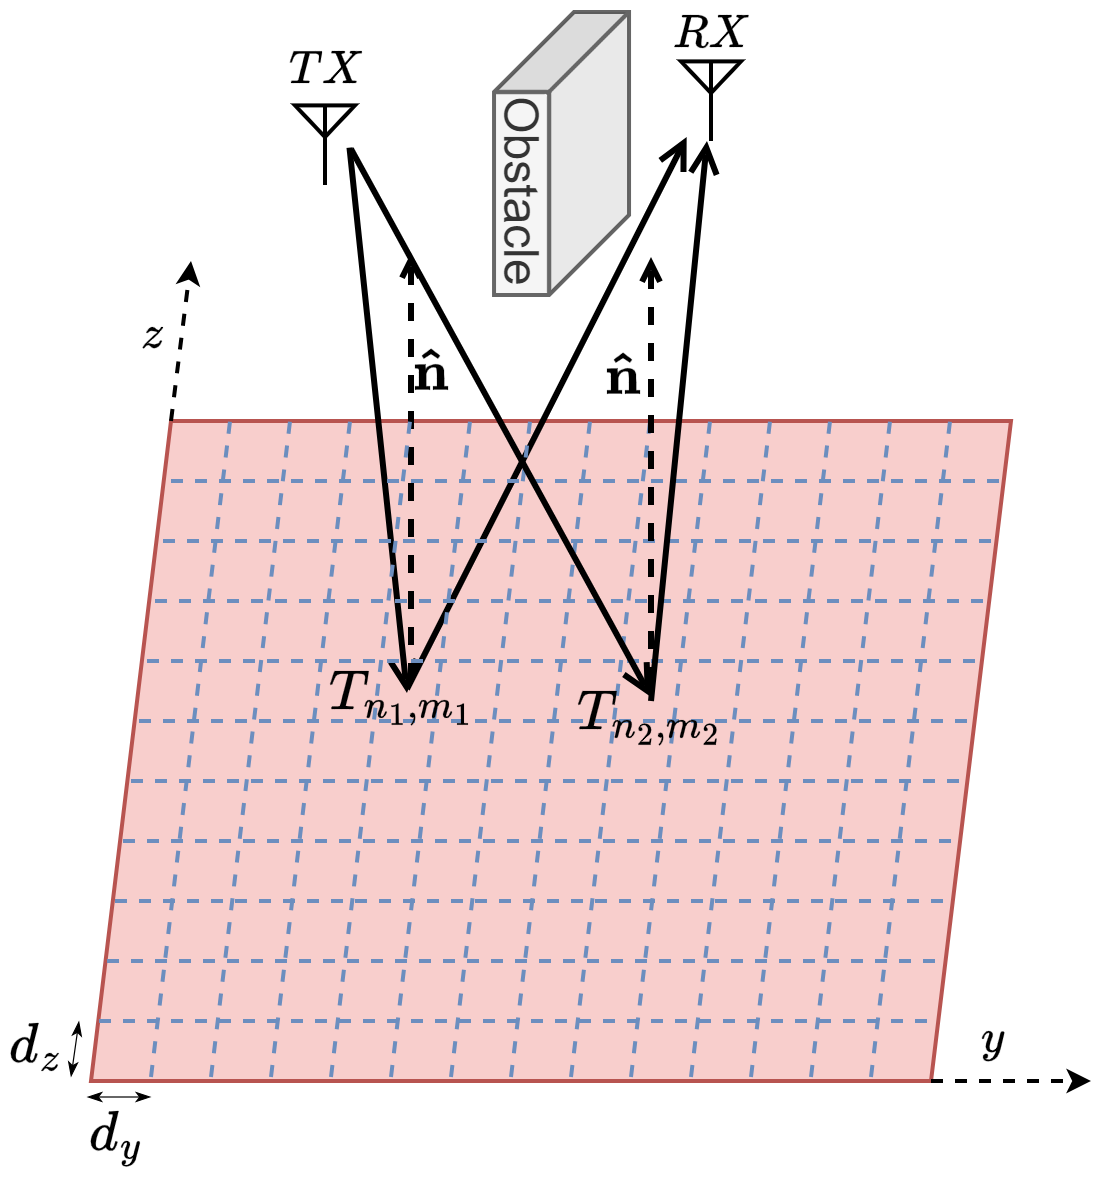
\includegraphics[width=.8\linewidth]{RIS_Modeling.png}
	\caption{Illustration of RIS modeling: The RIS surface is discretized into tiles, each with tunable reflection characteristics, to direct signals toward the desired target points.}
	\label{RIS_Modeling}
\end{figure}

\section{RIS PHASE PROFILE CONFIGURATION METHODS} \label{sec:phase_profile_section}
In RIS modeling, the primary focus is on the phase change introduced to the incoming signal, as the amplitude is typically assumed to remain constant, generally between $0.8$ and $1$. Therefore, the design and optimization of RIS are centered on assigning appropriate phase profiles to control the direction and behavior of reflected waves.

In this section, we consider two primary methods for configuring the phase profiles $\mathbf{\Phi}^k$ of the RIS to achieve anomalous reflections for each target point $k$: the gradient-based phase profile \cite{phase_grad_paper} and the distance-based phase profile \cite{Tang}. These methods offer distinct advantages, making them suitable for different environmental scenarios and system requirements.

\begin{enumerate}
	\item \textbf{Gradient-based Phase Profile}: This method considers the incidence and desired reflection wave directions, and it aims to achieve the desired reflection direction by introducing a phase gradient across the RIS. The phase gradient is computed to align the reflected signal with the desired reflection direction, thereby optimizing the coverage at the target points.
	
	\item \textbf{Distance-based Phase Profile}: In contrast to the gradient-based method, the distance-based method focuses on the total distance traveled by the incident and reflected signals. By adjusting the phase shifts to match the distances from the transmitter to each tile and from each tile to a specific target point, the method ensures that the reflected signals constructively interfere at this target point location.
\end{enumerate}

The phase profile for these methods is computed for each target point $k$, and the individual phase profiles are combined through the summation in (\ref{ref_coef_exp}) to derive the overall reflection coefficient profile $\mathbf{\Gamma}$.

\subsection{GRADIENT-BASED PHASE PROFILE}
The gradient-based method, as illustrated in Fig. \ref{RIS_Phase_Gradient}, treats the RIS as an ideal phase gradient reflector. The phase gradient is calculated based on the incident wave direction and the desired reflection direction for each target point. In this method, the RIS introduces a phase gradient that modifies the direction of the reflected waves, aiming to direct the reflected signal toward a desired target point.

Let us consider an incident wave with wave vector $\mathbf{\hat{k}}_i$ arriving at the center of the RIS at an incidence angle $\theta_i$ with respect to the RIS normal vector $\mathbf{\hat{n}}$. The desired reflection direction for the target point $k$ is represented by the reflection wave vector $\mathbf{\hat{k}}_r$ with a reflection angle $\theta_r$. The incident phase gradient due to the inclined wavefront is given by
\begin{equation} \label{grad_phi_i}
	\nabla \varphi_i = - k_0 \sin\theta_i \, \mathbf{\hat{k}}_i^p = - k_0 \, \textbf{P} \mathbf{\hat{k}}_i
\end{equation}
where $k_0 = 2 \pi / \lambda$ is the wavenumber and $\lambda$ is the wavelength. Here, $\mathbf{\hat{k}}_i^p$ represents the unit projection of the incident wave vector $\mathbf{\hat{k}}_i$ onto the plane of the RIS, and $\textbf{P}$ is the projection operator, where $\textbf{P} \mathbf{\hat{k}}_i = \sin\theta_i \, \mathbf{\hat{k}}_i^p$.

The RIS applies an additional phase gradient $\nabla \varphi_{RIS}$, which adjusts the reflection direction to achieve the desired angle $\theta_r$. Then, the reflection phase gradient $\nabla \varphi_r$ becomes
\begin{equation} \label{grad_phi}
	\nabla \varphi_r = \nabla \varphi_i + \nabla \varphi_{RIS}
\end{equation}
Similar to (\ref{grad_phi_i}), the reflection phase gradient $\nabla \varphi_r$ is expressed as
\begin{equation} \label{grad_phi_r}
	\nabla \varphi_r = - k_0 \ \sin\theta_r \ \mathbf{\hat{k}}_r^p = - k_0 \ \textbf{P} \mathbf{\hat{k}}_r
\end{equation}
where $\mathbf{\hat{k}}_r^p$ is the unit projection vector of the reflection wave vector \( \mathbf{\hat{k}}_r \) onto the RIS. By substituting (\ref{grad_phi_i}) and (\ref{grad_phi_r}) into (\ref{grad_phi}), we find the desired phase gradient onto the RIS to reflect the incoming wave with direction $\mathbf{\hat{k}}_i$ to the reflection wave with direction $\mathbf{\hat{k}}_r$
\begin{equation} \label{grad_exp}
	\nabla \varphi_{RIS} = k_0 \ \textbf{P} (\mathbf{\hat{k}}_i - \mathbf{\hat{k}}_r) = k_0 \ (\sin\theta_i \ \mathbf{\hat{k}}_i^p - \sin\theta_r \ \mathbf{\hat{k}}_r^p)
\end{equation}
For simpler cases, such as when the RIS, transmitter, and target positions are assumed to be at the same mounting height, the phase gradient onto the RIS becomes one-dimensional along the y-axis, which can be shown as follows:
\begin{equation} \label{grad_exp_simpler}
	\nabla \varphi_{RIS} = k_0 \, (\sin\theta_i - \sin\theta_r) \, \hat{y}
\end{equation}
This simplification results in a one-dimensional phase gradient and a more straightforward implementation of the RIS design.

To implement this gradient physically across the RIS, we initialize the phase to zero at the first RIS tile (e.g., the top-left corner) and apply a linear phase ramp across the surface according to the calculated gradient direction. For each tile $T_{n,m}$, the phase shift is computed by
\begin{equation}
	\varphi_{n,m}^k = \nabla \varphi_{RIS} \cdot (m \cdot d_y \, \hat{y} + n \cdot d_z \, \hat{z})
\end{equation}
where $d_y$ and $d_z$ are the RIS grid sizes along the $y$ and $z$ axes. This expression creates a structured linear phase variation over the array, effectively steering the reflected beam in the desired direction. This procedure is repeated for each target point $k$, and the resulting phase profile $\mathbf{\Phi}^k$ is then used to construct the RIS reflection coefficient via (\ref{ref_coef_exp}).
 
\begin{figure}
	\centering 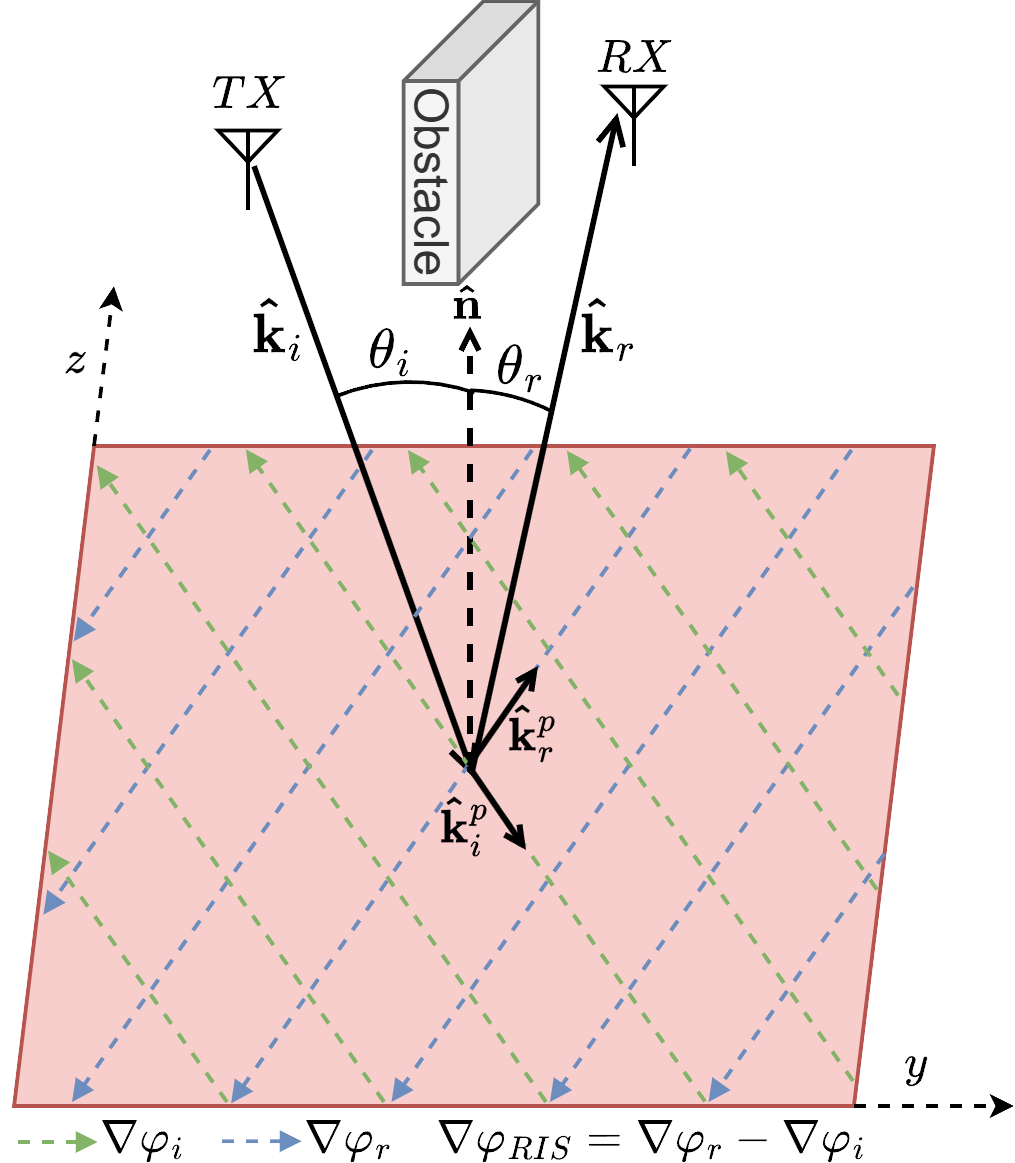
\includegraphics[width=.8\linewidth]{RIS_Phase_Gradient.png}
	\caption{The gradient-based method for configuring the RIS phase profile to reflect signals toward the target point}
	\label{RIS_Phase_Gradient}
\end{figure}

\subsection{DISTANCE-BASED PHASE PROFILE}
The distance-based method models the RIS as a focusing lens that ensures the reflected signals combine constructively at the target point. By calculating the phase shift required at each tile, this method ensures that the signals from all tiles travel the same total distance, ensuring constructive interference at the target point.

The position of each tile $T_{n,m}$ relative to the RIS center is given by $(0, (m-\frac{1}{2})d_y, (n-\frac{1}{2})d_z)$, where $m \in \left[ 1 - \frac{M}{2}, \frac{M}{2} \right]$ and $n \in \left[ 1 - \frac{N}{2}, \frac{N}{2} \right]$ represent the row and column indices of the tile, assuming that the center of the coordinate system is taken as the center of the RIS without loss of generality.

The electric field arriving at each tile $T_{n,m}$ is expressed as
\begin{equation}
	E_{n,m}^{\text{in}} = \sqrt{\frac{2 Z_0 P_{n,m}^{\text{TX-RIS}}}{d_y d_z}} e^{-j \frac{2 \pi r_{n,m}^{tx}}{\lambda}}
\end{equation}
where $Z_0$ is the characteristic impedance of free space, $r_{n,m}^{tx}$ is the distance between the transmitter and $T_{n,m}$, and $P_{n,m}^{\text{TX-RIS}}$ is the received power of the incident wave at each tile. After reflection, the total electric field at the desired target point is
\begin{equation}
	E^{rx} = \sum_{n=1-\frac{N}{2}}^{\frac{N}{2}} \sum_{m=1-\frac{M}{2}}^{\frac{M}{2}} E_{n,m}^{rx}
\end{equation}
where each reflected field, contributed by $T_{n,m}$ is:
\begin{equation} \label{E_n_m_r}
	E_{n,m}^{rx} = \sqrt{\frac{2 Z_0 P^{rx}_{n,m}}{A_{rx}}} e^{-j \left(\frac{2 \pi}{\lambda} (r_{n,m}^{tx} + r_{n,m}^{rx}) - \varphi_{n,m}^k\right)}
\end{equation}
where $r_{n,m}^{rx}$ is the distance from $T_{n,m}$ to the receiver, $A_{rx}$ is the receiving antenna aperture, and $P_{n,m}^{rx}$ is the power of the reflected signal of $T_{n,m}$ at the desired target point and can be expressed as
\begin{equation}
	P_{n,m}^{rx} = P_{n,m}^{\text{RIS-RX}} (A_{n,m}^k)^2 P_{n,m}^{\text{TX-RIS}}
\end{equation}
where $P_{n,m}^{\text{RIS-RX}}$ is the multiplicative factor to the received power of the path from $T_{n,m}$ to the desired target point. The combined received power of all tiles at target point $k$ is then given by
\begin{equation} \label{combined_rx_power}
	\begin{aligned}
		P^{rx} &= \frac{\left|E^{rx}\right|^2}{2 Z_0} A_{rx} \\
		&= \left| \sum_{n=1-\frac{N}{2}}^{\frac{N}{2}} \sum_{m=1-\frac{M}{2}}^{\frac{M}{2}} A_{n,m}^k \sqrt{P_{n,m}^{\text{TX-RIS}} P_{n,m}^{\text{RIS-RX}}} \right. \\
		&\quad \left. \times e^{-j \left(\frac{2 \pi}{\lambda} (r_{n,m}^{tx} + r_{n,m}^{rx}) - \varphi_{n,m}^k\right)} \right|^2
	\end{aligned}
\end{equation}
In the distance-based phase profile method, the aim is to maximize the combined received power $P^{rx}$ in (\ref{combined_rx_power}), which is maximized when the imaginary part of each term in the summation is tuned in. Then, the following phase assignment for each tile holds:
\begin{equation}
	\varphi_{n,m}^k = \frac{2 \pi}{\lambda} (r_{n,m}^{tx} + r_{n,m}^{rx})
\end{equation}
where the phase profile $\mathbf{\Phi}^k$ is created by assigning this expression to each tile to achieve constructive interference at the desired target point.

It is important to note that this phase profile is designed modulo $2\pi$, which inherently accounts for the periodic nature of phase. As a result, perfect path length equality is not required, constructive interference can still occur when path differences are integer multiples of the wavelength. Furthermore, environmental effects such as multipath propagation and higher-order reflections are automatically captured by the ray-tracing tool, which traces and aggregates all ray contributions. Therefore, the phase profile focuses on the dominant reflection path, while the full channel behavior is evaluated by the ray-tracing tool during simulation.

\section{JOINT RIS SIZE, POSITION AND TARGET POINT OPTIMIZATION ALGORITHM} \label{algo_section}
In this paper, the position of the transmitter is assumed to be fixed in the scene. Then, we can easily simulate the transmitter-only coverage map in the ray-tracing tool and reveal the scenario's blind spots with insufficient signal power that require coverage enhancement. The objective of this study is to utilize RIS deployment to improve the signal power in these blind spots, ensuring acceptable signal quality throughout all the areas in the scene.

In our previous work \cite{emre_claude_eucap_paper}, we addressed this issue by introducing a method to identify blind spots based on the transmitter-only coverage map. By defining a minimum power threshold for acceptable signal quality, regions with power levels below this threshold were classified as low-power cells which require coverage enhancement. The coordinates of these low-power cells were then grouped into a fixed number of clusters using the K-means clustering algorithm, and the centroids of these clusters were selected as the target points for the RIS. However, the position of the RIS in \cite{emre_claude_eucap_paper} was assumed to be fixed, which limited the flexibility of the solution.

To overcome this limitation, we propose a novel algorithm in this paper that jointly optimizes the RIS size, position, and number of target points. The algorithm first identifies low-power cells based on the transmitter-only coverage map. For each possible number of target points, it searches for feasible RIS positions within the scene that maintain a LoS connection with both the transmitter and all target points. Each feasible configuration of RIS position and number of target points is evaluated for each searched RIS size. The best configuration defined by the RIS position and number of target points is selected for each RIS size. Subsequently, the RIS size is varied iteratively, and the performance improvement is assessed. When the performance improvement falls below the defined threshold, the corresponding RIS size is selected as the sub-optimal size. This approach not only seeks to improve coverage but also balances performance gains with hardware cost by determining a sub-optimal RIS size. Increasing the RIS size enhances coverage, but after a certain point, the performance improvement becomes marginal compared to the added cost. Hence, the proposed algorithm identifies the trade-off point between performance and cost by defining a performance improvement threshold. This threshold manages the decision to continue increasing the RIS size. Without loss of generality, this study varies the RIS size by adjusting its width while keeping its height fixed, allowing for a clear analysis of one-dimensional size variations. However, the approach can be extended to two-dimensional size adjustments, where both height and width are increased proportionally. Detailed steps of the proposed algorithm are presented in two steps as Algorithm \ref{algo1} and Algorithm \ref{algo2}.

Although the algorithm employs an exhaustive search over discrete RIS width values, the computational cost is mitigated by two practical considerations. First, candidate RIS positions are pre-selected based on the requirement of line-of-sight connectivity to both the transmitter and all selected target points, reducing the search space significantly. Second, the RIS width is varied in decimeter level, making the number of evaluations manageable even in large indoor scenarios. Nevertheless, in cases where finer resolution (e.g., millimeter-level granularity) is required or the deployment environment is significantly larger, several strategies can be considered to enhance scalability:
\begin{itemize}
	\item Heuristic search strategies, such as greedy algorithms,
	\item Early stopping, where the search terminates if performance improvement falls below a selected performance improvement threshold,
	\item Coarse-to-fine grid search, where RIS width candidates are sampled more sparsely at first, followed by local refinement around the best region,
	\item Analytical bounds based on coverage radius or path geometry to prune unpromising regions.
\end{itemize}
In fact, our algorithm already includes an early stopping mechanism via a minimum performance improvement threshold. This allows the algorithm to terminate the search once further increases in RIS width no longer produce significant performance improvements in the performance metric compared to the selected threshold. If finer search resolution is desired, this approach can be combined with the additional strategies mentioned above for further computational efficiency.

\begin{algorithm}
	\caption{Ray-tracing Based RIS Size, Position and Target Points Optimization (Part 1)}
	\label{algo1}
	\SetAlgoLined
	\KwIn{
		\begin{itemize}
			\item \textbf{The scene geometry:} A 3D representation of the area where coverage is to be enhanced, including obstacles, walls, etc.
			\item \textbf{Transmitter (TX) position:} Coordinates of the transmitter in the scene.
			\item \textbf{Minimum power threshold} $P_{\text{th}}$: The threshold for acceptable signal power, below which cells are considered low-power.
			\item \textbf{Range of possible target points} $\mathcal{N}$: The set of possible cluster counts to be used in K-means algorithm, e.g., $\mathcal{N} = \{1, 2, \dots, 5\}$.
			\item \textbf{Set of possible RIS widths} $\mathcal{W}$: The set of candidate RIS widths, e.g., $\mathcal{W} = \{0.2, 0.4, \dots, 3.0\}$ m.
			\item \textbf{Minimum performance improvement threshold} $\Delta \mathcal{M}_{\text{min}}$: The minimum performance improvement required to justify increasing the RIS width.
		\end{itemize}
	}
	\KwOut{
		\begin{itemize}
			\item \textbf{Sub-optimal number of target points} $N^{\text{opt}}$.
			\item \textbf{Sub-optimal RIS width} $W_{\text{RIS}}^{\text{opt}}$.
			\item \textbf{Sub-optimal RIS position} $\mathbf{r}_{\text{RIS}}^{\text{opt}}$.
		\end{itemize}
	}
	Compute the transmitter-only coverage map $\mathbf{P}_{\text{TX}}(x, y)$.\\
	Set a minimum power threshold $P_{\text{th}}$ for acceptable signal quality.\\
	Identify low-power cells in $\mathbf{P}_{\text{TX}}(x, y)$ where the power level is below the minimum power threshold $P_{\text{th}}$, denoted as $\mathcal{C}_{\text{low}}$:
	\begin{equation}
		\mathcal{C}_{\text{low}} = \{(x, y) \ | \ \mathbf{P}_{\text{TX}}(x, y) < P_{\text{th}}\}
	\end{equation}
\end{algorithm}

\begin{algorithm}
	\caption{Ray-tracing Based RIS Size, Position and Target Points Optimization (Part 2)}
	\label{algo2}
	\SetAlgoLined
	\ForEach{number of target points $N \in \mathcal{N}$}{
		Apply K-means algorithm to $\mathcal{C}_{\text{low}}$ to group the low-power cells into $N$ clusters and obtain $N$ centroids:
		\begin{equation}
			\text{K-means}(N, \mathcal{C}_{\text{low}}) \rightarrow \text{Centroids} \{ \mathbf{c}_1, \mathbf{c}_2, \dots, \mathbf{c}_N \}
		\end{equation}
		where each centroid $\mathbf{c}_i$ represents a target point where coverage enhancement is needed.\\
		Identify the set of feasible RIS positions $\mathcal{R}_N$ that provide LoS to both the transmitter and all $N$ target points:
		\begin{equation}
			\mathcal{R}_N = \{ \mathbf{r}_{\text{RIS}} \mid \text{LoS}(\mathbf{r}_{\text{RIS}}, \mathbf{TX}) \land \text{LoS}(\mathbf{r}_{\text{RIS}}, \mathbf{c}_i) \ \forall \mathbf{c}_i \}
		\end{equation}
		\ForEach{RIS width $W_{\text{RIS}} \in \mathcal{W}$}{
			Compute the combined coverage $\textbf{P}_{\text{comb}}(x,y)$ at each low-power cell, considering both TX and RIS contributions, for each RIS position $\mathbf{r}_{\text{RIS}} \in \mathcal{R}_N$.\\
			Calculate the performance metric $\mathcal{M}(\mathbf{r}_{\text{RIS}}, N, W_{\text{RIS}})$ for all parameter combinations as the average power of low-power cells after placing the RIS at $\mathbf{r}_{\text{RIS}}$:
			\begin{equation}
				\mathcal{M}(\mathbf{r}_{\text{RIS}}, N, W_{\text{RIS}}) = \frac{1}{|\mathcal{C}_{\text{low}}|} \sum_{(x, y) \in \mathcal{C}_{\text{low}}} \mathbf{P}_{\text{comb}}(x, y)
			\end{equation}
		}
	}
	
	Identify the RIS configuration $(\mathbf{r}_{\text{RIS}}^{W_{\text{RIS}}}, N^{W_{\text{RIS}}}, W_{\text{RIS}})$ that maximizes the performance metric $\mathcal{M}$ for each $W_{\text{RIS}}$:
	\begin{equation}
		(\mathbf{r}_{\text{RIS}}^{W_{\text{RIS}}}, N^{W_{\text{RIS}}}) = \arg\max_{\mathbf{r}_{\text{RIS}} \in \mathcal{R}_N, N \in \mathcal{N}} \mathcal{M}(\mathbf{r}_{\text{RIS}}, N, W_{\text{RIS}})
	\end{equation}\\
	Select the smallest RIS width $W_{\text{RIS}}^{\text{opt}}$ for which increasing the RIS width further does not yield a performance improvement exceeding $\Delta \mathcal{M}_{\text{min}}$. Assign corresponding parameters $\mathbf{r}_{\text{RIS}}^{\text{opt}} = \mathbf{r}_{\text{RIS}}^{W_{\text{RIS}}^{\text{opt}}}$ and $N^{\text{opt}} = N^{W_{\text{RIS}}^{\text{opt}}}$.
\end{algorithm}

\section{SIMULATION RESULTS} \label{sec:results}
This section presents comprehensive simulation results to evaluate the effectiveness of the proposed RIS placement optimization algorithm for indoor wireless coverage enhancement. We begin by describing the simulation scenario and introducing the developed graphical user interface (GUI) that facilitates the extraction and visualization of simulation results. We then outline the simulation parameters used throughout our experiments.

The results are organized progressively, starting with the transmitter-only coverage map that establishes our baseline, followed by detailed analyses for two different minimum power thresholds. For each threshold, we present binary poor coverage maps for different numbers of target points, optimization algorithm results for varying RIS configurations, cumulative distribution function analyses of power levels, and combined coverage analyses with RIS deployment. Through these results, we demonstrate how RIS placement significantly improves signal coverage in blind spots and enhances overall system performance across the indoor environment.

\subsection{SIMULATION SCENARIO}
In this paper, we consider a U-shaped indoor office scenario consisting of three main hallways: the `upper' and `lower' hallways, which form the two arms of the U, and the `intersecting' hallway that connects them at the bottom. Additionally, there is an internal room located at the intersection of these hallways. The layout of the scenario is illustrated in Fig. \ref{Scenario}, where the transmitter position is marked with a blue circle, and an example RIS placement is represented by a purple rectangle on the intersecting hallway wall.

For the simulation environment, the materials used for the walls, floors, and ceilings are selected from a predefined list in Sionna RT, based on their typical usage in indoor environments and their electromagnetic properties. Sionna RT incorporates material models defined in the ITU-R P.2040-2 recommendation \cite{ITU}. Specifically, the selected materials are:  
\begin{itemize}
	\item \textbf{Walls:} Plasterboard (\textit{itu\_plasterboard}) is chosen due to its common application in building interiors.
	\item \textbf{Floors:} Chipboard (\textit{itu\_chipboard}) is selected for its suitability and practicality as an indoor flooring material.
	\item \textbf{Ceilings:} Ceiling board (\textit{itu\_ceiling\_board}) is used for its specific design for ceilings.
\end{itemize}

In this scenario, the transmitter is assumed to be placed at the intersection of the hallways on the upper side, as indicated by the blue circle in Fig. \ref{Scenario}. This placement may result in potential blind spots with weak signal quality at the far edge of the lower hallway and certain areas within the internal room. To mitigate these blind spots, a RIS can be strategically positioned on the wall of the intersecting hallway, depending on the selected minimum power threshold value.

\begin{figure}
	\centering 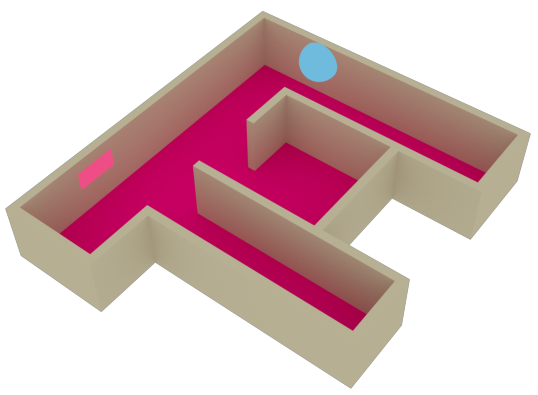
\includegraphics[width=.8\linewidth]{Sim_Results/Scenario_Illustration.png}
	\caption{Scenario Illustration}
	\label{Scenario}
\end{figure}

\subsection{GRAPHICAL USER INTERFACE (GUI) FOR SIMULATION RESULTS EXTRACTION}
A Python-based graphical user interface (GUI) has been developed to facilitate the extraction and visualization of simulation results for the proposed algorithm. The main interface of this GUI is shown in Fig. \ref{GUI}. This interface allows users to load predefined scenarios, define the operating frequency of the scene, set the position of the transmitter, specify the minimum power threshold, and configure numerous other parameters.

After the necessary parameters are entered, the GUI provides several functionalities, including generating coverage map plots, identifying the RIS target points, based on the distribution of low-power cells in the transmitter-only coverage map and displaying feasible RIS positions depending on the location of the target points.

Furthermore, the GUI allows users to define the boundaries for optimization parameters related to the proposed algorithm in Section \ref{algo_section}. These parameters include the number of target points, RIS width, and RIS position. The GUI computes performance metrics for all possible combinations of these parameters, enabling users to end up with sub-optimal optimization configurations. Additionally, the GUI can visualize the effect of RIS width on performance metrics, as well as generate cumulative distribution functions (CDFs) for different phase profile approaches and RIS sizes.

\begin{figure}
	\centering 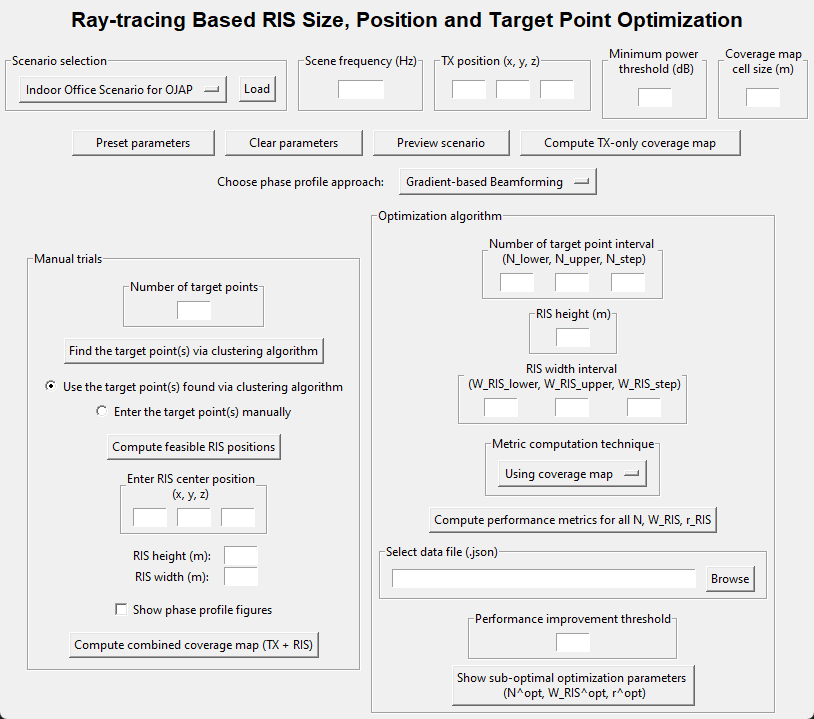
\includegraphics[width=\linewidth]{Sim_Results/GUI.png}
	\caption{Illustration of the GUI interface}
	\label{GUI}
\end{figure}

\subsection{SIMULATION PARAMETERS}
The simulation parameters are carefully chosen to evaluate the performance of the proposed algorithm under realistic conditions. The key simulation parameters used throughout this study are summarized in Table \ref{tab:sim_params}. Unless otherwise specified, the amplitude profile of the reflection coefficients for each target point is set to unity in all simulations to isolate and analyze the pure effect of the phase profiles. This assumption simplifies the RIS design and is widely adopted in RIS literature. To further assess its validity, we also include an evaluation of random amplitude fluctuations in Figures \ref{amp_change_comb_cov_gradient} and \ref{amp_change_comb_cov_distance}, where the amplitude of each tile is randomly drawn from a uniform distribution between $0.7$ and $1$. The results confirm that such fluctuations have a negligible effect on performance in the considered scenarios. The power intensity coefficients, $c_k$, which determine how power is distributed among the target points, are set to equal values, ensuring identical importance is assigned to each blind spot in the scenario.

The system operates at a communication frequency of $5.8$ GHz, corresponding to a wavelength of $\lambda = c/f = 5.17$ cm, where $c$ is the speed of light. The RIS grid sizes, $d_y$ and $d_z$, are defined as $\lambda / 2 = 2.585$ cm, which is a commonly adopted configuration in ray-tracing simulations and RIS literature. This choice ensures that the array operates within the subwavelength regime, preventing grating lobes while maintaining effective wavefront manipulation and high beamforming efficiency.

In this study, the mounting heights of the RIS, transmitter, and target points are all fixed at $1.5$ m to allow fair comparison of coverage performance under equal elevation conditions. This mounting height is used to compute the path gain coverage map with the ray-tracing tool. However, this assumption does not restrict the generality of the proposed RIS optimization framework. If different mounting heights are considered for the RIS or other nodes, the ray-tracing tool can generate a new coverage map reflecting those geometry changes, and our optimization algorithm can operate on the new map without any changes to its structure. Throughout this paper, we refer to the vertical aperture size of the RIS as the “RIS height,” while the z-axis elevation of its center is termed the “mounting height.”

The resolution of the simulated coverage maps are controlled by three key parameters provided by the Sionna RT coverage map computation method:
\begin{itemize}
	\item \texttt{max\_depth}, which defines the maximum number of path bounces to trace,
	\item \texttt{cm\_cell\_size}, which sets the physical dimensions of each grid cell in the map,
	\item \texttt{num\_samples}, the number of rays traced through the scene.
\end{itemize}
Higher values of \texttt{num\_samples} and \texttt{max\_depth}, and smaller values of \texttt{cm\_cell\_size}, lead to more detailed results but also increase simulation time. In our simulations, we selected \texttt{max\_depth} = 6, \texttt{cm\_cell\_size} = [0.4, 0.4] m, and \texttt{num\_samples} = 20,000,000, which we found to offer a good trade-off between runtime and coverage accuracy. These parameters are scenario-dependent and can be adjusted as needed; however, they do not affect the robustness of the proposed RIS optimization algorithm, which operates reliably across different coverage map resolutions.

The power levels in the coverage maps are measured in dBW, normalized to a unit transmit power of $1$ W. This simplifies the analysis to focus on relative path loss rather than absolute transmit power, ensuring consistency with common ray-tracing practices. For brevity, values are denoted as `dB' in figures and text, with the understanding that they represent dBW relative to 1 W transmit power.

Two distinct minimum power threshold values $P_{\text{th}}$ are considered in the simulations:  
\begin{itemize}
	\item $-100$ dB: This threshold results in a higher number of low-power cells in the scene, providing a broader area for the RIS to enhance.
	\item $-110$ dB: This lower threshold value allows the RIS to focus on cells with comparably weaker power levels.
\end{itemize}

The results corresponding to these threshold values are simulated separately to assess the impact of power thresholds on the optimization and coverage enhancement provided by the RIS.

\begin{table}[t]
	\centering
	\caption{Key simulation parameters}
	\begin{tabular}{l l}
		\toprule
		\textbf{Parameter} & \textbf{Value} \\
		\midrule
		Communication frequency & $5.8$ GHz \\
		Wavelength ($\lambda$) & $5.17$ cm \\
		RIS grid sizes ($d_y$, $d_z$) & $2.585$ cm ($\lambda/2$) \\
		Mounting height (Tx, RIS, target points) & $1.5$ m \\
		Path gain threshold ($P_{\text{th}}$) & $-100$ dB and $-110$ dB \\
		\underline{Sionna RT-related parameters:} & \\
		Max ray tracing depth (\texttt{max\_depth}) & 6 reflections \\
		Coverage map resolution (\texttt{cm\_cell\_size}) & $0.4$ m × $0.4$ m \\
		Number of traced rays (\texttt{num\_samples}) & 20,000,000 \\
		\bottomrule
	\end{tabular}
	\label{tab:sim_params}
\end{table}

\subsection{TRANSMITTER-ONLY COVERAGE MAP}
The transmitter-only coverage map, which represents the power distribution from the transmitter without the assistance of a RIS, is depicted in Fig. \ref{TX_coverage_map}. The transmitter position is marked with a red `+' sign. As observed in the figure, signal power decreases significantly in certain areas of the scenario, resulting in potential blind spots with weak signal coverage.

Specifically, these blind spots are primarily located at the far edge of the lower hallway and in several regions within the internal room. The presence of these blind spots highlights the limitations of transmitter-only coverage in complex indoor environments with NLoS regions and significant signal attenuation caused by obstacles and walls. Such weak coverage can negatively impact the reliability and quality of communication in these areas.

To address these limitations, the strategic placement of a RIS becomes essential. By redirecting and enhancing the signal, the RIS can extend the coverage to include these blind spots, thereby improving the overall system performance. The selection of an optimal RIS placement depends on factors such as the distribution of the low-power cells in the blind spots and the minimum power threshold values used in the simulations.

Fig. \ref{TX_coverage_map} serves as the baseline coverage map, against which the improvements brought by the RIS placement and optimization will be evaluated in subsequent sections.

\begin{figure}
	\centering 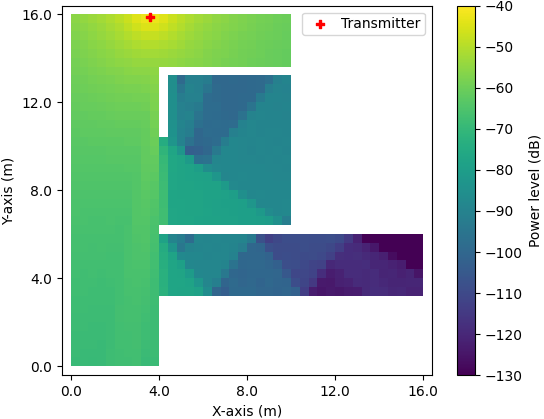
\includegraphics[width=\linewidth]{Sim_Results/TX_coverage_map.png}
	\caption{Transmitter-only coverage map}
	\label{TX_coverage_map}
\end{figure}

\subsection{RESULTS FOR MINIMUM POWER THRESHOLD OF $-100$ dB}

\subsubsection{BINARY POOR COVERAGE MAPS FOR DIFFERENT NUMBER OF TARGETS}
We begin by assigning a minimum power threshold of $-100$ dB. As explained earlier, cells in the coverage map that fall below this threshold are categorized as low-power cells, which require a power boost for reliable communication. The distribution of these low-power cells is depicted in Fig. \ref{binary_maps} for different numbers of target points $N$. These plots, referred to as binary poor coverage maps, visually represent the areas where the signal strength is below the threshold (red areas) and areas where the signal strength is acceptable (blue areas).

The positions of the low-power cells are clustered using the K-means algorithm, and the centroids of these clusters are marked as green `$\times$' symbols in Fig. \ref{binary_maps}. These centroids represent the target points where the RIS will steer its beams to improve signal coverage. Feasible RIS positions are then determined based on LoS visibility to both the target points and the transmitter. These positions are indicated by green star symbols on the same figure.

For each configuration shown in Fig. \ref{binary_maps}, the average power of the low-power cells is calculated as $-112.58$ dB, significantly below the set minimum power threshold of $-100$ dB.

In addition to the average power of the low-power cells, we also analyze a new metric known as the coverage ratio. The coverage ratio represents the percentage of the scene that is covered by either the transmitter or the RIS. The coverage ratio in the transmitter-only coverage map for the consideration of the minimum power threshold of $-100$ dB is $81.54\%$, as seen in Fig. \ref{binary_maps}. This metric is crucial, as focusing only on the average power of low-power cells might lead to misleading results. For example, a higher average power could indicate an improvement in performance, but if many areas remain uncovered, the coverage ratio could still be limited. A situation like this might arise if the RIS concentrates on boosting the power of certain low-power cells, thus increasing their signal strength significantly, while leaving other low-power cells uncovered. Monitoring the coverage ratio reveals such scenarios and helps ensure that the optimization does not overlook areas that still lack coverage. Although this issue can occur, it is generally rare because the RIS initially boosts the power level of any low-power cell it illuminates. However, after a certain point, focusing further on the same cell does not result in exponential power increases, as the RIS effect becomes saturated.

\begin{figure}
	\centering
	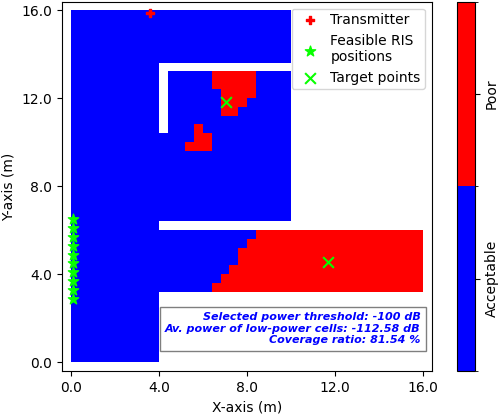
\includegraphics[width=0.49\linewidth]{Sim_Results/Binary_Cov_Map_N_2_-100dB.png}
	\hfill
	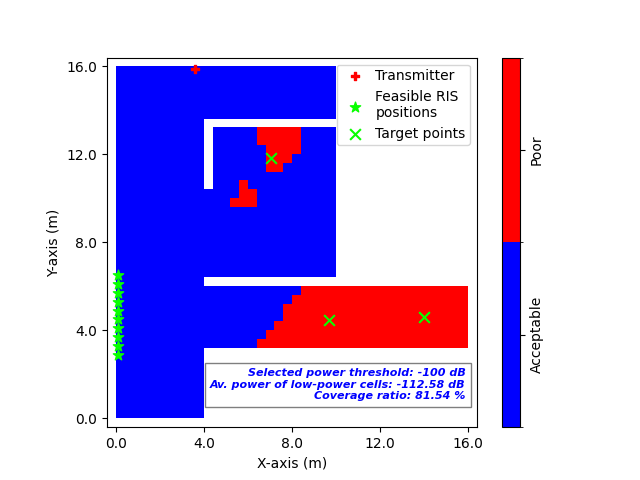
\includegraphics[width=0.49\linewidth]{Sim_Results/Binary_Cov_Map_N_3_-100dB.png}
	
	a) $N = 2$ \hspace{80pt} b) $N = 3$ \\[5pt]
	
	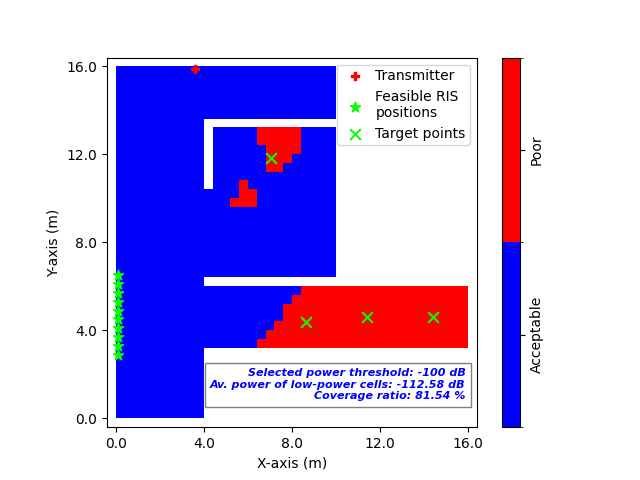
\includegraphics[width=0.49\linewidth]{Sim_Results/Binary_Cov_Map_N_4_-100dB.png}
	\hfill
	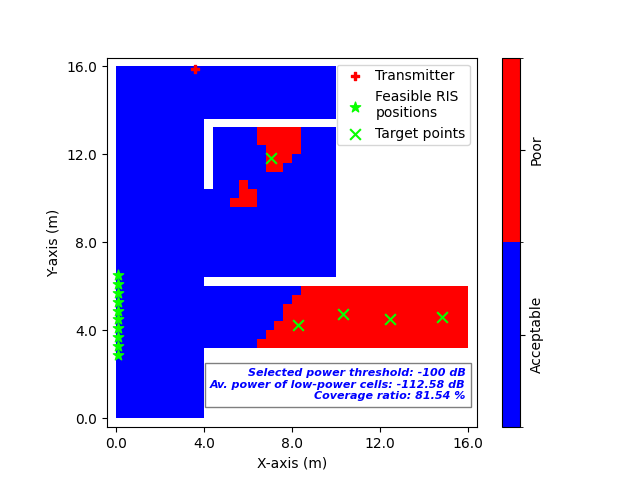
\includegraphics[width=0.49\linewidth]{Sim_Results/Binary_Cov_Map_N_5_-100dB.png}
	
	c) $N = 4$ \hspace{80pt} d) $N = 5$
	\caption{Binary poor coverage maps for different number of target configurations for the minimum power threshold of $-100$ dB}
	\label{binary_maps}
\end{figure}

\subsubsection{RIS OPTIMIZATION ALGORITHM RESULTS}
After mapping low-power areas and determining target points and feasible RIS positions, we apply our optimization algorithm (Section \ref{algo_section}) to compute the performance metric $\mathcal{M}$ over various parameters: number of targets, RIS positions, and RIS width. For each RIS width, the configuration that maximizes $\mathcal{M}$ is identified as the sub-optimal configuration for that specific width.

Fig. \ref{perf_metric_RIS_width_multiple_curves_-100dB} shows $\mathcal{M}$ versus RIS width for different RIS heights and two phase profile approaches. It can be observed that the curves tend to saturate beyond a certain RIS width. Initially, increasing RIS width significantly improves low-power coverage, however, once most cells reach acceptable power, further width increases yield little benefit, which highlights the need for cost-effectiveness.

Another notable observation is that the gradient-based approach consistently outperforms the distance-based approach for the considered minimum power threshold of $-100$ dB. This is because the gradient-based approach not only boosts the power at the target points but also increases the power at other locations along the beam paths, covering a broader area. In contrast, the distance-based approach aims to create constructive interference specifically at the target points, which results in a more localized effect. While this approach leads to a significant power boost at the selected points, it does not effectively extend coverage to surrounding low-power cells, leaving some areas insufficiently illuminated. Despite this limitation, the distance-based approach still yields a noticeable improvement in performance. This difference between these phase profile approaches is particularly seen in scenarios where the low-power regions are large, making the gradient-based approach more effective in such cases.

The impact of RIS height is also more noticeable in the distance-based approach compared to the gradient-based approach. Specifically, when the RIS height is increased from $0.5$ m to $1$ m, the improvement in performance is more significant for the distance-based approach. In contrast, for the gradient-based approach, a smaller RIS height provides nearly equivalent performance, suggesting that a lower RIS height can be selected in such cases to balance performance with practical deployment constraints.

\begin{figure}
	\centering
	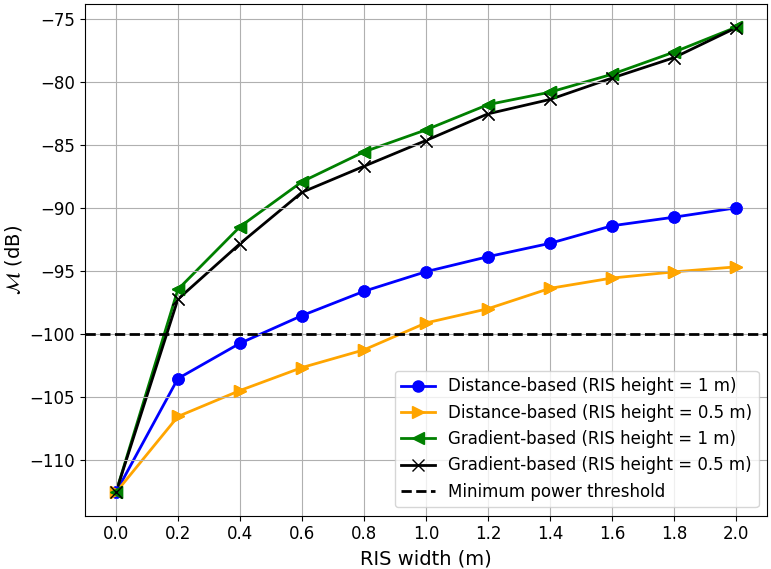
\includegraphics[width=\linewidth]{Sim_Results/perf_metric_RIS_width_multiple_curves_-100dB.png}
	\caption{Performance metric $\mathcal{M}$ as a function of RIS width for different RIS heights and phase profile approaches, with a minimum power threshold of $-100$ dB}
	\label{perf_metric_RIS_width_multiple_curves_-100dB}
\end{figure}

Next, in Fig. \ref{perf_metric_RIS_width_-100dB_gradient_height_1m}, the gradient-based approach for a RIS height of $1$ m is analyzed in detail. The figure highlights the RIS configurations that maximize the performance metric $\mathcal{M}$ for each RIS width. The annotations in the figure indicate the optimal RIS positions (denoted as “RIS pos”) and the number of target points for different widths as well as the corresponding coverage ratio. 

To determine the sub-optimal RIS width, a performance improvement threshold $\Delta \mathcal{M}_{\text{min}}$ is introduced. This threshold represents the minimum performance gain required to justify increasing the RIS width to the next level. Higher thresholds lead to smaller RIS widths with slightly reduced performance, as increasing the RIS width further does not provide sufficient improvement to justify the additional cost. As seen in Fig. \ref{perf_metric_RIS_width_-100dB_gradient_height_1m}, even a minimal RIS width of $0.2$ m significantly boosts $\mathcal{M}$ compared to the No RIS case. Furthermore, the coverage ratio improves significantly, reaching nearly $100\%$ at larger RIS widths, demonstrating the effectiveness of the optimization algorithm.

Also, the number of target points are assigned less and less with increasing the RIS width. This is because initially, the RIS width is not enough to cover the large area of blind spots, that's why the RIS is assigned to more number of target points to cover all of the region. However, after increasing the RIS width, since the thickness of the beam from the RIS increases, it becomes sufficient to obtain better performance results with a less number of targets without dividing the power allocated to each target point.

\begin{figure}
	\centering
	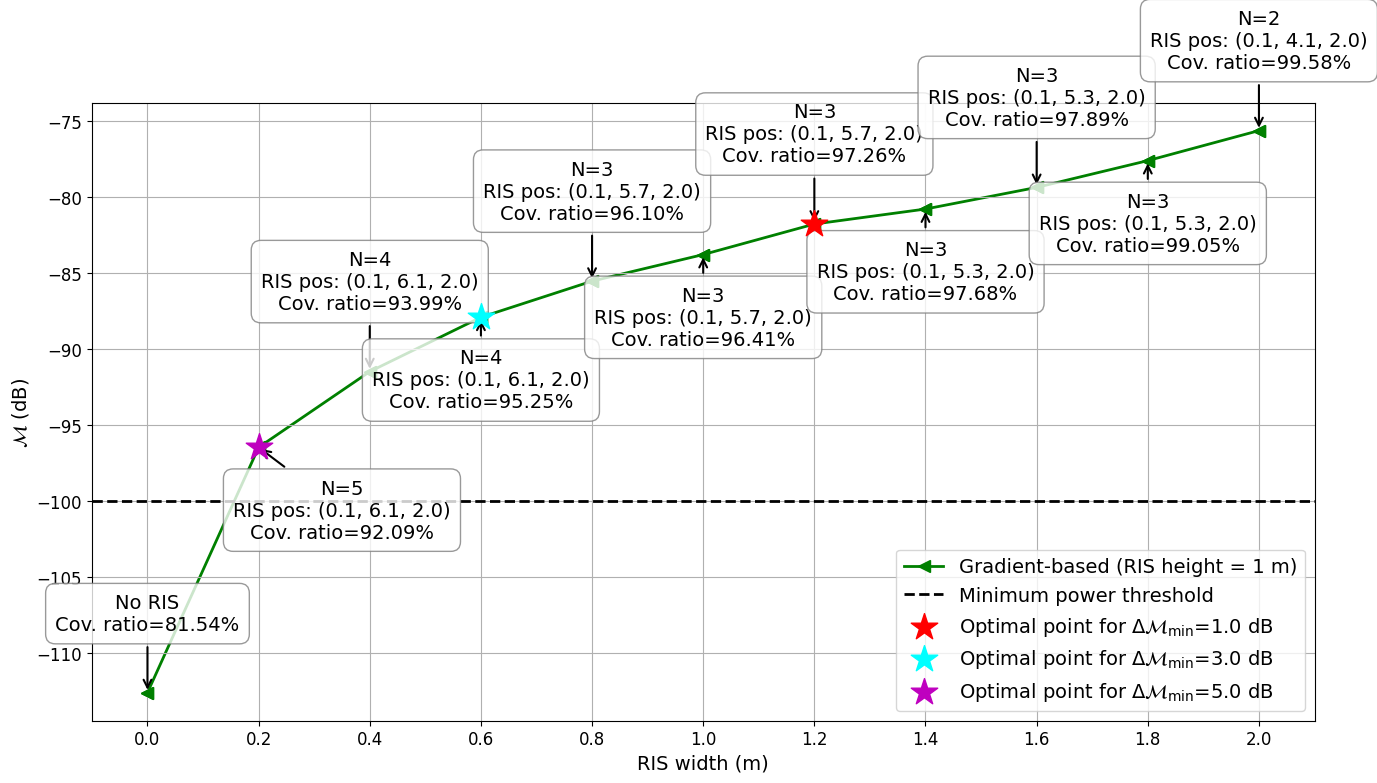
\includegraphics[width=\linewidth]{Sim_Results/perf_metric_RIS_width_-100dB_gradient_height_1m.png}
	\caption{Performance metric $\mathcal{M}$ vs. RIS width for the gradient-based approach, showing selected sub-optimal configurations for different performance improvement thresholds $\Delta \mathcal{M}_{\text{min}}$ with a RIS height of $1$ m and a minimum power threshold of $-100$ dB}
	\label{perf_metric_RIS_width_-100dB_gradient_height_1m}
\end{figure}

In Fig. \ref{perf_metric_RIS_width_-100dB_distance_height_1m}, the distance-based approach is analyzed for a RIS height of $1$ m. Similar trends are observed, with slightly lower performance metric values and coverage ratios compared to the gradient-based approach. This difference reflects the distance-based approach’s narrower focus on the target points, which leaves some low-power cells uncovered.

\begin{figure}
	\centering
	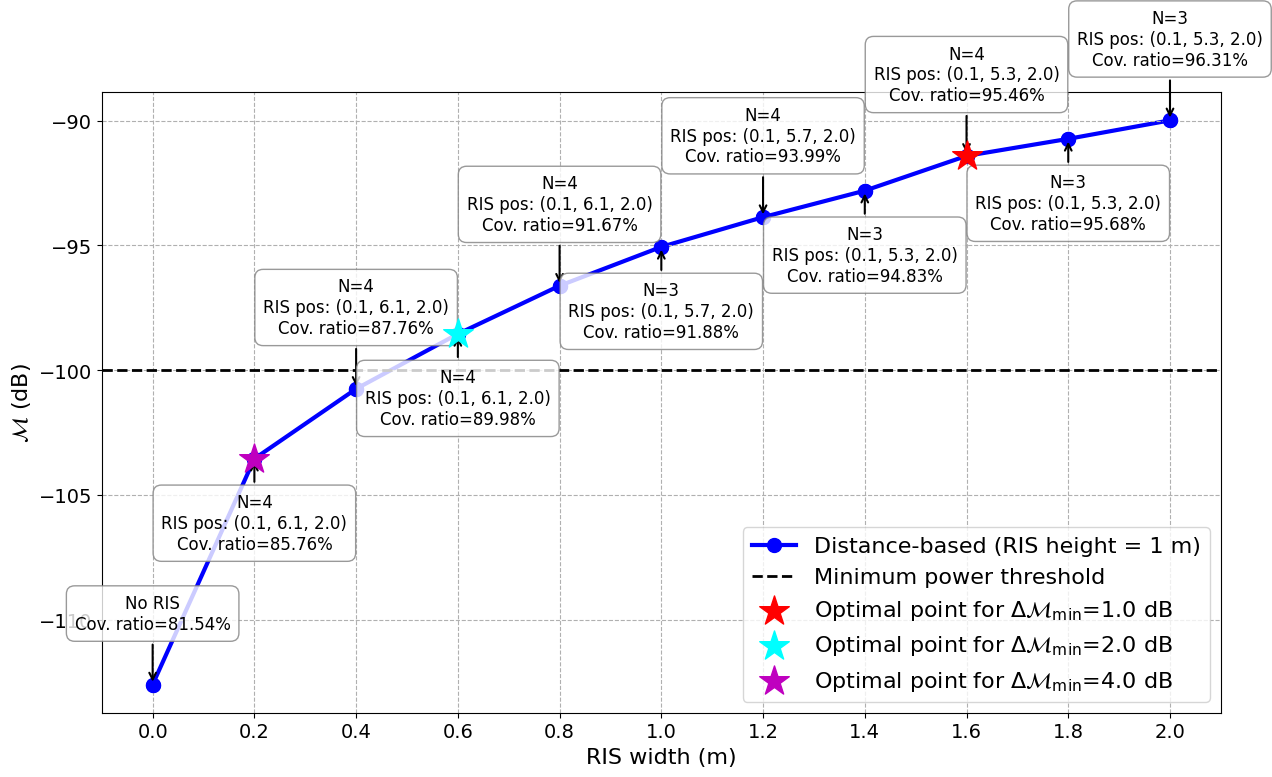
\includegraphics[width=\linewidth]{Sim_Results/perf_metric_RIS_width_-100dB_distance_height_1m.png}
	\caption{Performance metric $\mathcal{M}$ vs. RIS width for the distance-based approach, showing selected sub-optimal configurations for different performance improvement thresholds $\Delta \mathcal{M}_{\text{min}}$ with a RIS height of $1$ m and a minimum power threshold of $-100$ dB}
	\label{perf_metric_RIS_width_-100dB_distance_height_1m}
\end{figure}

\subsubsection{EFFECT OF NUMBER OF TARGET POINTS ON THE PERFORMANCE}
To directly analyze the influence of the number of target points $N$ on the performance, Figures \ref{performance_and_coverage_vs_N_Gradient} and \ref{performance_and_coverage_vs_N_Distance} show the variation in the performance metric \(\mathcal{M}\) and coverage ratio for two fixed RIS widths: $1$ m and $2$ m. These are plotted for the gradient-based and distance-based approaches, separately.

Each plot includes solid lines for the performance metric and dashed lines for the coverage ratio. For each value of $N$, the RIS configuration with the highest performance metric (among all candidate positions) is selected. The corresponding RIS position is annotated at each point using 3D coordinates $(x, y, z)$. Fig. \ref{binary_poor_cov_map_N_1} shows the binary poor coverage map for the case of $N=1$, where the target point selected by the K-means clustering algorithm is marked with a green `$\times$'.

In the gradient-based case (Fig. \ref{performance_and_coverage_vs_N_Gradient}), the performance metric $\mathcal{M}$ increases significantly from $N = 0$ (no RIS) to $N = 2$, reflecting the fact that two distinct blind spot regions exist in the considered indoor scenario. However, further increases in the number of target points provide negligible performance gains, as most uncovered regions have already been served with $N = 2$. For RIS width $W_{\text{RIS}} = 1$ m, the optimal number of target points is $N = 3$, whereas for $W_{\text{RIS}} = 2$ m, $N = 2$ is sufficient. This difference is explained due to the fact that a larger RIS width allows energy to reach a wider area with fewer number of target points. The coverage ratio, on the other hand, continues to improve with increasing $N$, since more target points distribute energy more broadly, which allows more low-power cells to benefit from the RIS contribution.

In the distance-based case (Fig. \ref{performance_and_coverage_vs_N_Distance}), similar behavior is observed. The only difference is that this time the optimal number of target points is $3$ for both $W_{\text{RIS}}$ values. This is because the distance-based approach focuses energy in a narrower area, meaning that more number of target points would be needed compared to the gradient-based approach to cover the same number of low-power cells.

These results demonstrate that the number of RIS target points should be selected based on the width of the RIS and the geometry of blind-spot regions. Selecting too few targets can leave areas unserved, while selecting too many reduces the power directed toward each.

\begin{figure}
	\centering 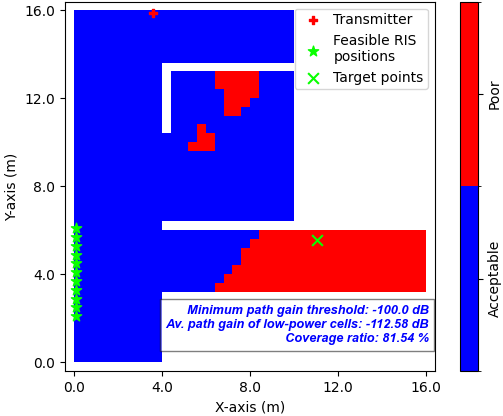
\includegraphics[width=.7\linewidth]{Sim_Results/Binary_Cov_Map_N_1_-100dB.png}
	\caption{Binary poor coverage map with $N = 1$ for the minimum path gain threshold of $-100$ dB}
	\label{binary_poor_cov_map_N_1}
\end{figure}

\begin{figure}
	\centering
	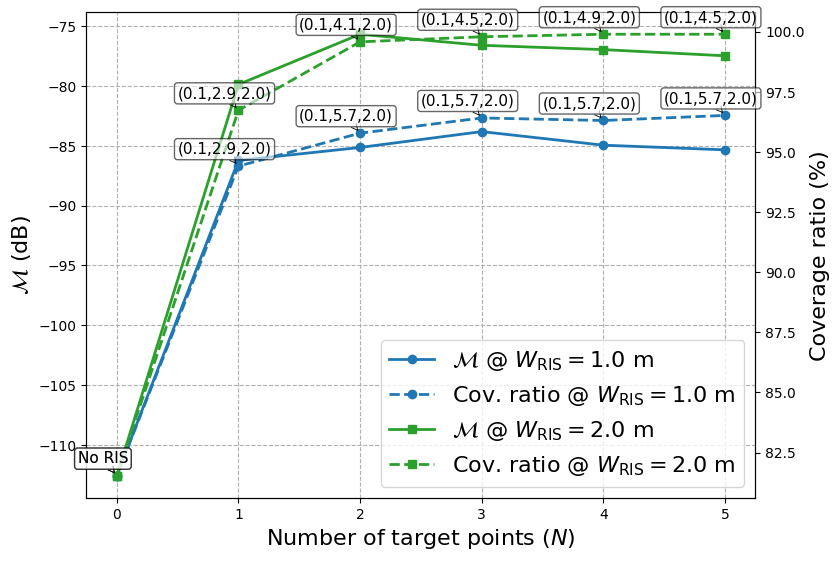
\includegraphics[width=\linewidth]{Sim_Results/performance_and_coverage_vs_N_Gradient.png}
	\caption{Performance metric $\mathcal{M}$ vs. number of target points ($N$) for the gradient-based approach, with a RIS height of $1$ m and a minimum path gain threshold of $-100$ dB where each point is annotated with the corresponding optimal RIS position in the form $(x, y, z)$}
	\label{performance_and_coverage_vs_N_Gradient}
\end{figure}

\begin{figure}
	\centering
	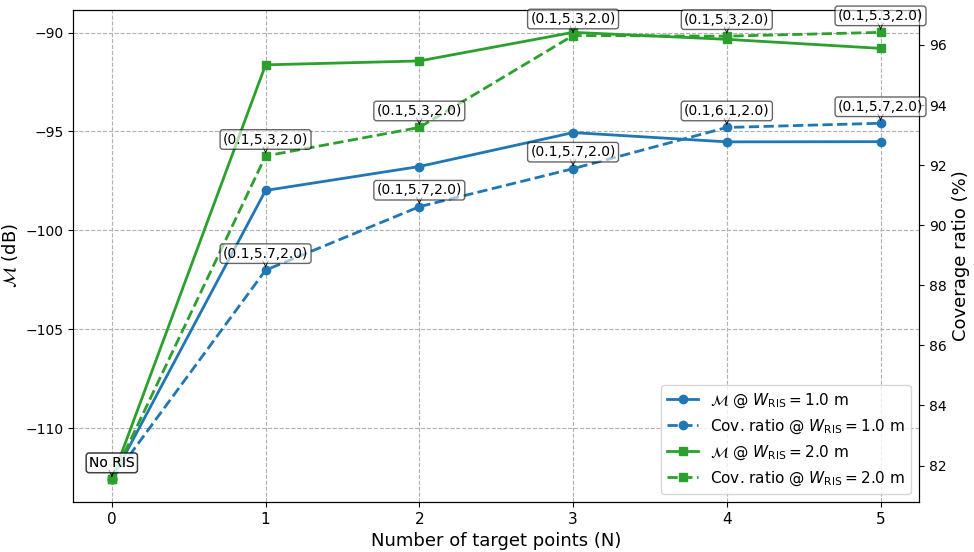
\includegraphics[width=\linewidth]{Sim_Results/performance_and_coverage_vs_N_Distance.png}
	\caption{Performance metric $\mathcal{M}$ vs. number of target points ($N$) for the distance-based approach, with a RIS height of $1$ m and a minimum path gain threshold of $-100$ dB where each point is annotated with the corresponding optimal RIS position in the form $(x, y, z)$}
	\label{performance_and_coverage_vs_N_Distance}
\end{figure}

\subsubsection{CUMULATIVE DISTRIBUTION FUNCTION (CDF) ANALYSIS OF POWER LEVELS IN THE SCENE}
To evaluate the impact of RIS placement on overall power distribution, we analyze the CDF of the power levels across the entire scene for different phase profile approaches and RIS sizes, as shown in Fig. \ref{CDF_-100dB}. The RIS is positioned at its sub-optimal location for each size, as identified in Figs. \ref{perf_metric_RIS_width_-100dB_gradient_height_1m} and \ref{perf_metric_RIS_width_-100dB_distance_height_1m}. In the figure labels, the RIS size is denoted in the format `height × width'.

The results indicate that the lowest power levels in the scene are significantly improved by both the distance-based and gradient-based approaches compared to the baseline case without RIS. This is because the RIS primarily targets low-power cells in blind spots, where signal coverage is weakest. The key difference between the two approaches is observed in the moderate power level range. While the gradient-based approach enhances power levels in these cells considerably, the distance-based approach exhibits a more localized effect, focusing primarily on the designated target points. Nevertheless, even the distance-based approach provides noticeable enhancement compared to the no RIS scenario in the case of $-100$ dB minimum power threshold.

Furthermore, increasing the RIS size for the distance-based approach improves the power of the low-power cells. However, for moderate power level cells, the performance variation between different RIS size cases is negligible. For the gradient-based approach, performance improvements persist across moderate power level cells as well, since a larger RIS size allows for broader coverage of surrounding areas. This difference arises because the gradient-based approach not only optimizes power at the target points but also contributes to enhancing the power levels of neighboring cells, whereas the distance-based approach maintains a more focused strategy.

As expected, high-power-level cells remain unaffected by the RIS placement since they are already well covered by the transmitter, and the RIS does not specifically target these areas. This observation further emphasizes that the RIS primarily benefits low-power and moderate-power regions, rather than areas that are already sufficiently illuminated by the direct transmitter signal.

\begin{figure}
	\centering 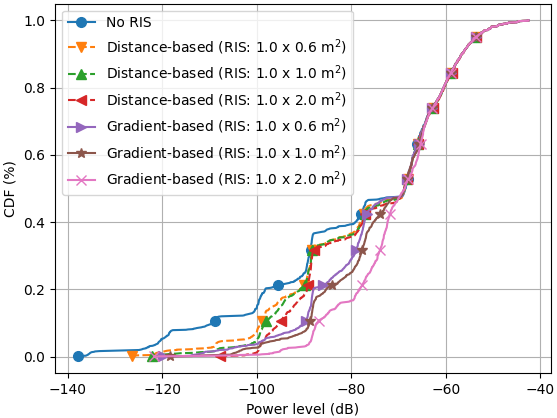
\includegraphics[width=\linewidth]{Sim_Results/CDF_-100dB.png}
	\caption{Cumulative distribution functions (CDFs) of power levels for different phase profile approaches and RIS sizes, with a minimum power threshold of $-100$ dB}
	\label{CDF_-100dB}
\end{figure}

\subsubsection{COMBINED COVERAGE ANALYSIS WITH RIS}
To further evaluate the impact of RIS placement, we analyze the combined coverage maps of the transmitter and the RIS for a specific configuration. Fig.s \ref{comb_cov_gradient} and \ref{comb_cov_distance} illustrate the results for the gradient-based and distance-based approaches, respectively.

Fig. \ref{comb_cov_gradient} presents the results for the gradient-based approach, where the RIS is configured with a size of $1 \times 2$ m$^2$ and positioned at its sub-optimal location, as identified in Fig. \ref{perf_metric_RIS_width_-100dB_gradient_height_1m}. The RIS serves two target points, marked by red `$\times$' signs, while its placement is indicated by a star symbol. The combined coverage map in Fig. \ref{comb_cov_gradient}-a demonstrates that the RIS successfully enhances the power levels at the target points while also improving signal strength along the beam paths. To better quantify this enhancement, the RIS coverage gain in Fig. \ref{comb_cov_gradient}-b highlights significant power level improvements, particularly at the far edge of the lower hallway and within the internal room where the target points are located. Finally, Fig. \ref{comb_cov_gradient}-c shows the updated binary poor coverage map, demonstrating that nearly all cells achieve sufficient power coverage, with a coverage ratio of $99.58\%$ and an increased average power of low-power cells reaching $-76.05$ dB compared to a coverage ratio of $81.54\%$ and an average power of low-power cells of $-112.58$ dB in the transmitter-only coverage map. Figs. \ref{comb_cov_gradient}-d and \ref{comb_cov_gradient}-e illustrate the per-tile phase profiles generated by the gradient-based method for each target point in this RIS configuration. As seen, the method produces a linear phase ramp across the RIS surface to steer the reflected beams toward the assigned target directions. In this scenario, RX-1 refers to the receiver point inside the internal room, while RX-2 is located in the lower corridor region.

\begin{figure}
	\centering
	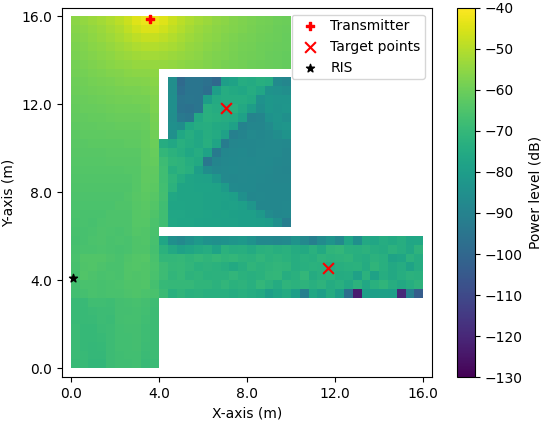
\includegraphics[width=0.8\linewidth]{Sim_Results/Comb_cov_1x2_Gradient.png}
	
	a) Combined coverage map \\[5pt]
	
	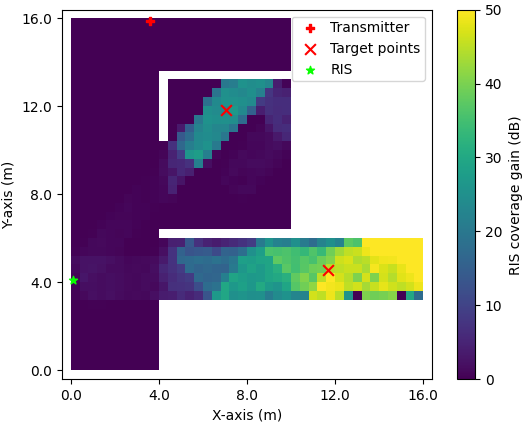
\includegraphics[width=0.49\linewidth]{Sim_Results/RIS_cov_gain_1x2_Gradient.png}
	\hfill
	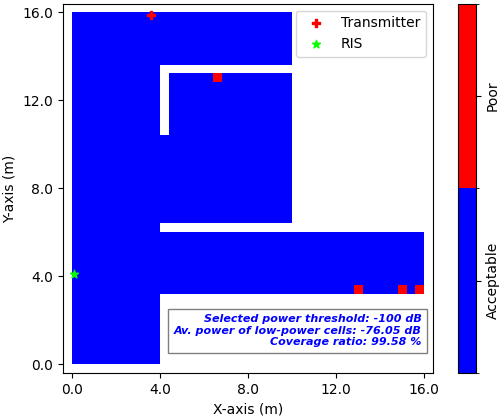
\includegraphics[width=0.48\linewidth]{Sim_Results/New_Binary_Cov_Map_1x2_Gradient.png}
	
	\hspace{10pt} b) RIS coverage gain \hspace{30pt} c) Updated binary poor \\ \hspace{140pt} coverage map \\[5pt]

	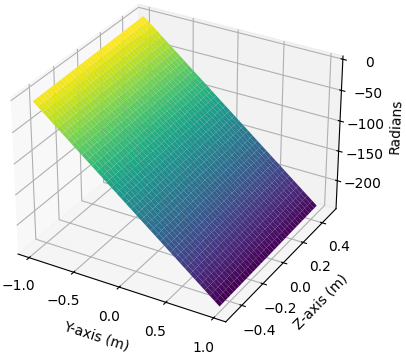
\includegraphics[width=0.48\linewidth]{Sim_Results/pp_-100dB_gradient_RX1.png}
	\hfill
	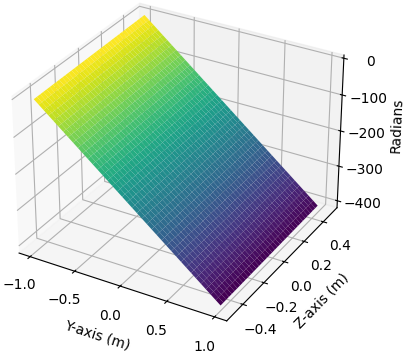
\includegraphics[width=0.48\linewidth]{Sim_Results/pp_-100dB_gradient_RX2.png}
	
	\hspace{10pt} d) Phase profile for RX-1 \hspace{15pt} e) Phase profile for RX-2
	\caption{Combined coverage analysis for a RIS of size $1 \times 2$ m$^2$ using the gradient-based approach, with a minimum power threshold of $-100$ dB}
	\label{comb_cov_gradient}
\end{figure}

A similar analysis is conducted for the distance-based approach, as illustrated in Fig. \ref{comb_cov_distance}. The RIS configuration follows the sub-optimal parameters obtained from the optimization algorithm. As shown in Fig. \ref{comb_cov_distance}, the distance-based approach directs energy to narrow regions around the target points. Unlike the gradient-based approach, this method does not significantly enhance power levels outside the focused target point areas. Consequently, some low-power cells, particularly in the large blind spot of the lower hallway, remain uncovered despite the RIS placement. This outcome is specific to the given scenario, where a large blind spot region exists, however, in cases with smaller blind spot areas, the distance-based approach could also yield superior results. Nevertheless, the binary poor coverage map in Fig. \ref{comb_cov_distance}-c indicates that the average power of low-power cells increases to $-89.6$ dB, with a gain of nearly $23$ dB, while the coverage ratio of the scene reaches $96.31\%$. Figs. \ref{comb_cov_distance}-d, \ref{comb_cov_distance}-e, and \ref{comb_cov_distance}-f show the per-tile phase profiles generated by the distance-based method for each of the three optimally selected target points in this configuration. Unlike the gradient-based method, the distance-based method produces nonuniform and focused phase distributions that precisely align the total TX–RIS–target path lengths. This results in energy being concentrated narrowly around each target point, making the method particularly effective for small or well-isolated blind-spot regions.

This highlights the trade-offs between the two approaches. While the gradient-based approach provides a more distributed power enhancement, the distance-based approach focuses energy more precisely on the assigned target points. The performance of these methods may also depend on the scenario, as we will explore in the next subsection by lowering the minimum power threshold to $-110$ dB to focus on the weakest signal regions.

\begin{figure}
	\centering
	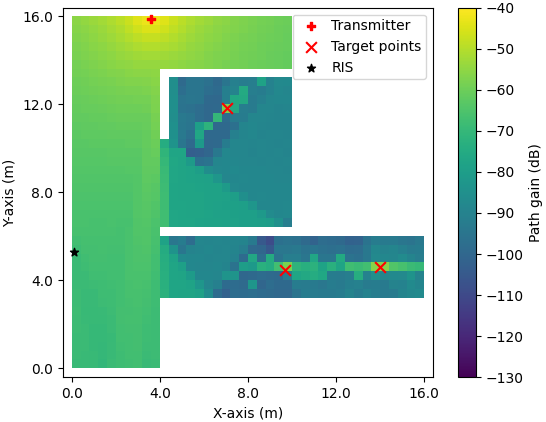
\includegraphics[width=0.8\linewidth]{Sim_Results/Comb_cov_1x2_Distance.png}
	
	a) Combined coverage map \\[5pt]
	
	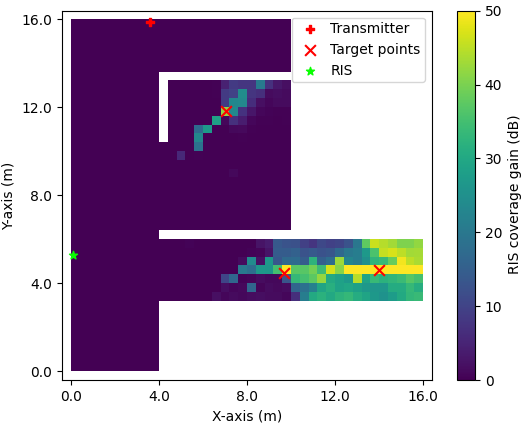
\includegraphics[width=0.49\linewidth]{Sim_Results/RIS_cov_gain_1x2_Distance.png}
	\hfill
	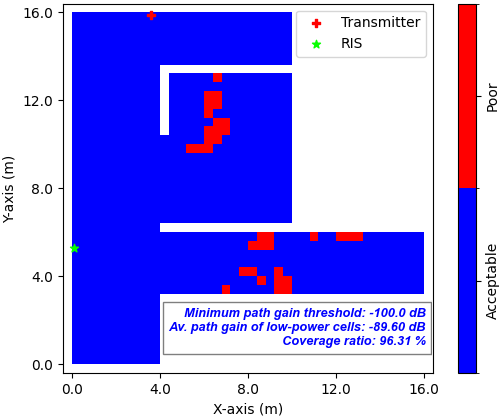
\includegraphics[width=0.48\linewidth]{Sim_Results/New_Binary_Cov_Map_1x2_Distance.png}
	
	\hspace{10pt} b) RIS coverage gain \hspace{30pt} c) Updated binary poor \\ \hspace{140pt} coverage map
	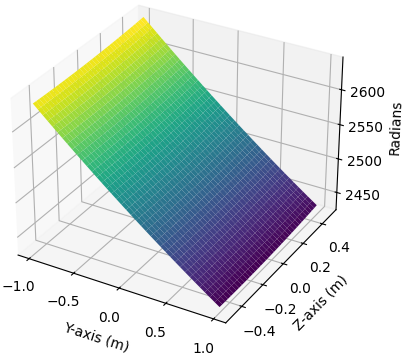
\includegraphics[width=0.48\linewidth]{Sim_Results/pp_-100dB_distance_RX1.png}
	\hfill
	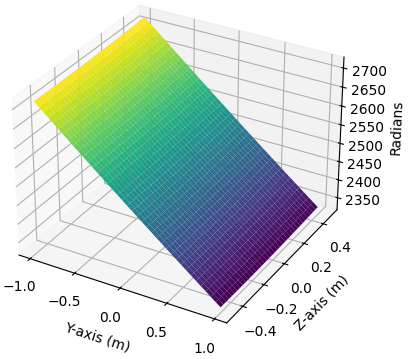
\includegraphics[width=0.48\linewidth]{Sim_Results/pp_-100dB_distance_RX2.png}

	\hspace{10pt} d) Phase profile for RX-1 \hspace{15pt} e) Phase profile for RX-2 \\[5pt]
	
	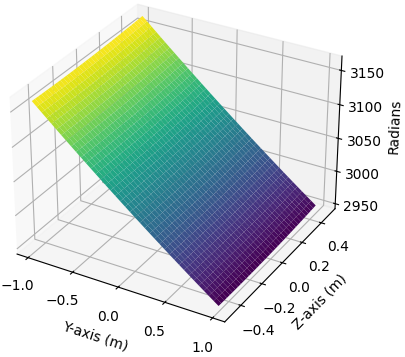
\includegraphics[width=0.49\linewidth]{Sim_Results/pp_-100dB_distance_RX3.png}
	
	f) Phase profile for RX-3
	
	\caption{Combined coverage analysis for a RIS of size $1 \times 2$ m$^2$ using the distance-based approach, with a minimum power threshold of $-100$ dB}
	\label{comb_cov_distance}
\end{figure}

\subsubsection{EFFECT OF AMPLITUDE FLUCTUATIONS ON RIS PERFORMANCE}
In this subsection, we analyze the impact of random amplitude fluctuations across RIS tiles on the coverage and system performance. To this end, we conducted a simulation by introducing random fluctuations in the amplitude profile of the RIS tiles. In this case only, each element’s amplitude for a given target point was independently assigned from a uniform distribution between $0.7$ and $1$. This setup approximates practical fluctuations observed in passive RIS implementations due to angular-dependent attenuation or fabrication variability.

Figures \ref{amp_change_comb_cov_gradient} and \ref{amp_change_comb_cov_distance} present the resulting coverage maps and performance metrics using the gradient-based and distance-based approaches, respectively. These results are generated using the same RIS configurations as in Figures \ref{comb_cov_gradient} and \ref{comb_cov_distance}. The results reveal that both approaches are largely robust to moderate amplitude variations. Specifically, the average path gain of the low-power cells drops by only $1$–$1.5$ dB compared to the fixed-unit amplitude case. The coverage patterns also remain largely unchanged, with no significant degradation observed in the combined coverage or binary poor coverage maps. This indicates that the system performance is predominantly determined by the phase configuration rather than fine-grained amplitude tuning. As such, fixed amplitude assumptions are sufficient for capturing the dominant effects of RIS behavior in phase-driven optimization frameworks, particularly when the RIS operates passively and angular-dependent attenuation is weak. Nonetheless, future work could further explore this aspect by incorporating angle-dependent amplitude profiles, particularly in scenarios involving hardware-calibrated RIS models or where amplitude distortions are non-negligible.

\begin{figure}
	\centering
	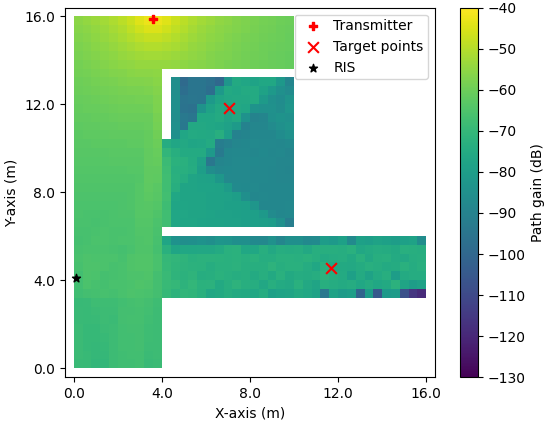
\includegraphics[width=0.8\linewidth]{Sim_Results/amp_change_Comb_cov_1x2_Gradient.png}
	
	a) Combined coverage map \\[5pt]
	
	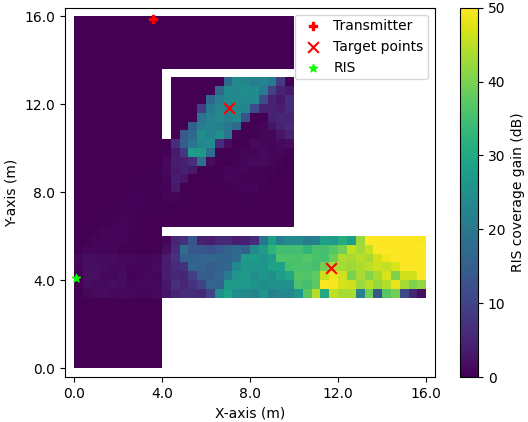
\includegraphics[width=0.49\linewidth]{Sim_Results/amp_change_RIS_cov_gain_1x2_Gradient.png}
	\hfill
	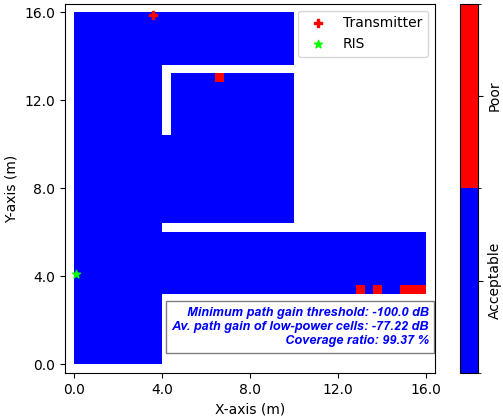
\includegraphics[width=0.48\linewidth]{Sim_Results/amp_change_New_Binary_Cov_Map_1x2_Gradient.png}
	
	\hspace{10pt} b) RIS coverage gain \hspace{30pt} c) Updated binary poor \\ \hspace{140pt} coverage map
	\caption{Combined coverage analysis for a RIS of size $1 \times 2$ m$^2$ using the gradient-based approach with random amplitude fluctuations (uniformly distributed in [$0.7$, $1$]), under a minimum path gain threshold of $-100$ dB.}
	\label{amp_change_comb_cov_gradient}
\end{figure}

\begin{figure}
	\centering
	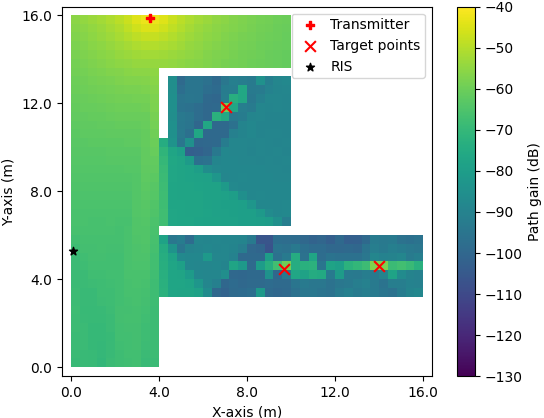
\includegraphics[width=0.8\linewidth]{Sim_Results/amp_change_Comb_cov_1x2_Distance.png}
	
	a) Combined coverage map \\[5pt]
	
	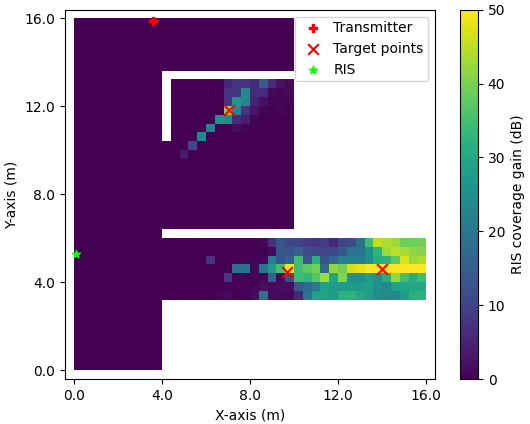
\includegraphics[width=0.49\linewidth]{Sim_Results/amp_change_RIS_cov_gain_1x2_Distance.png}
	\hfill
	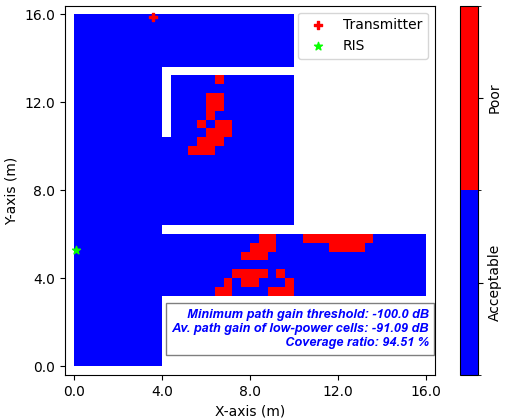
\includegraphics[width=0.48\linewidth]{Sim_Results/amp_change_New_Binary_Cov_Map_1x2_Distance.png}
	
	\hspace{10pt} b) RIS coverage gain \hspace{30pt} c) Updated binary poor \\ \hspace{140pt} coverage map
	\caption{Combined coverage analysis for a RIS of size $1 \times 2$ m$^2$ using the distance-based approach with random amplitude fluctuations (uniformly distributed in [$0.7$, $1$]), under a minimum path gain threshold of $-100$ dB.}
	\label{amp_change_comb_cov_distance}
\end{figure}

\subsection{RESULTS FOR MINIMUM POWER THRESHOLD OF $-110$ dB}
In this subsection, we analyze the impact of reducing the minimum power threshold to $-110$ dB, focusing on the weakest signal regions and their blind spots. This analysis follows a similar methodology to the $-100$ dB case but reveals different outcomes due to the updated power threshold.

Fig. \ref{binary_maps_-110dB} presents the binary poor coverage maps for different numbers of target configurations when the minimum power threshold is set at $-110$ dB. The low-power cells in this setting are primarily located at the far edge of the lower hallway, whereas the previously identified low-power cells within the internal room are no longer present. This is because the power levels in that region predominantly fall between $-100$ dB and $-110$ dB, making them non-critical under the new threshold. Consequently, the RIS optimization now focuses only on the far edge of the lower hallway with a smaller blind spot region. Considering only the transmitter's contribution, the average power of these newly identified low-power cells is calculated as $-121.87$ dB, with an initial coverage ratio of $90.40\%$.

\begin{figure}
	\centering
	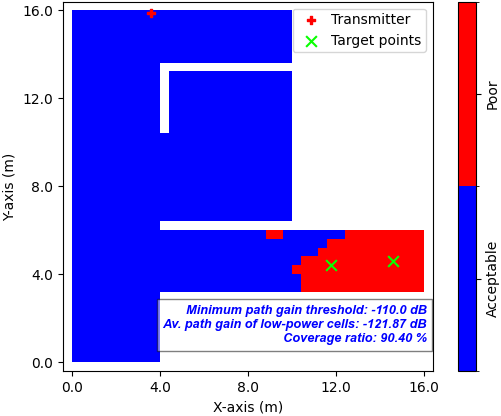
\includegraphics[width=0.49\linewidth]{Sim_Results/Binary_Cov_Map_N_2_-110dB.png}
	\hfill
	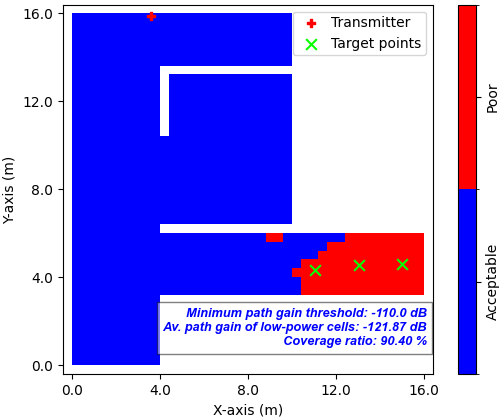
\includegraphics[width=0.49\linewidth]{Sim_Results/Binary_Cov_Map_N_3_-110dB.png}
	
	a) $N = 2$ \hspace{80pt} b) $N = 3$ \\[5pt]
	
	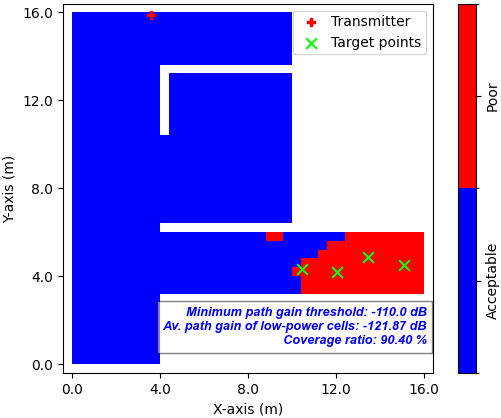
\includegraphics[width=0.49\linewidth]{Sim_Results/Binary_Cov_Map_N_4_-110dB.png}
	\hfill
	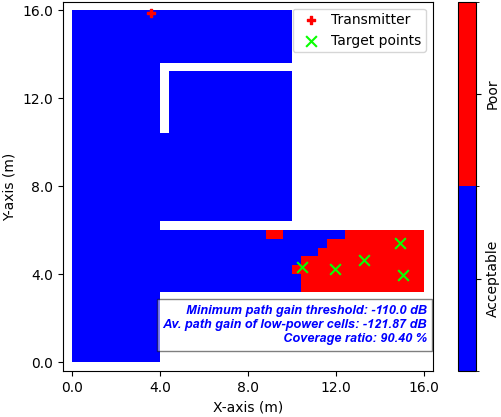
\includegraphics[width=0.49\linewidth]{Sim_Results/Binary_Cov_Map_N_5_-110dB.png}
	
	c) $N = 4$ \hspace{80pt} d) $N = 5$
	\caption{Binary poor coverage maps for different number of target configurations for the minimum power threshold of $-110$ dB}
	\label{binary_maps_-110dB}
\end{figure}

Following the identification of new low-power cells and their corresponding target points, we execute RIS placement and performance evaluations across all feasible locations using the proposed optimization algorithm. Similar to the previous case, the results of the performance metric $\mathcal{M}$ as a function of RIS width are illustrated in Fig. \ref{perf_metric_RIS_width_-110dB_multiple_curves_height_1m}, comparing gradient-based and distance-based approaches. Given the fewer number of low-power cells, all located within the same blind spot, satisfactory coverage improvement is achieved even with a relatively small RIS width for both approaches. While the coverage ratio reaches nearly $100\%$ for most RIS configurations, the gradient-based approach still provides a higher average power level for the low-power cells compared to the distance-based approach.

\begin{figure}
	\centering 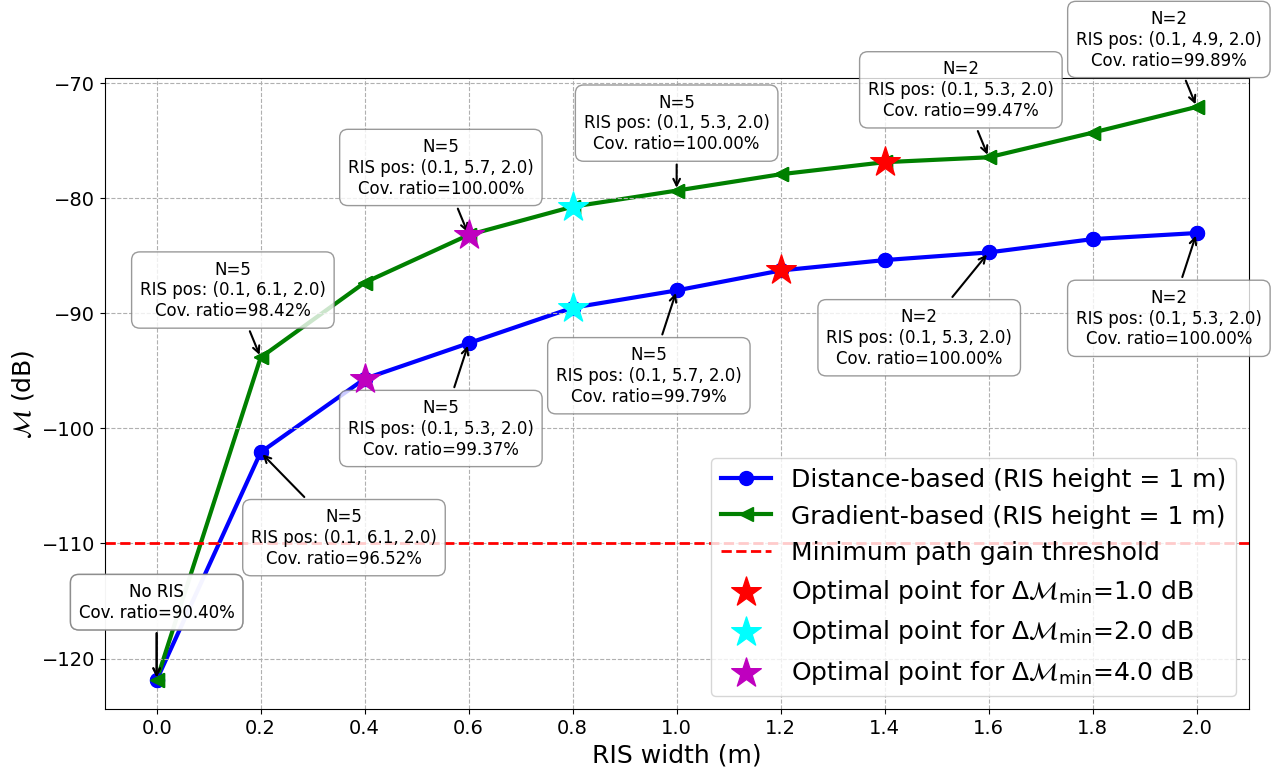
\includegraphics[width=\linewidth]{Sim_Results/perf_metric_RIS_width_-110dB_multiple_curves_height_1m.png}
	\caption{Performance metric $\mathcal{M}$ vs. RIS width plot, showing selected sub-optimal configurations for different performance improvement thresholds $\Delta \mathcal{M}_{\text{min}}$ with a RIS height of $1$ m and a minimum power threshold of $-110$ dB}
	\label{perf_metric_RIS_width_-110dB_multiple_curves_height_1m}
\end{figure}

The CDFs of power levels for different phase profile approaches and RIS sizes with a minimum power threshold of $-110$ dB are presented in Fig. \ref{CDF_-110dB}. The observed trends are consistent with the previous CDF analysis for the $-100$ dB case. The major distinction in this scenario is that the lowest-power cells are almost entirely served with the RIS placement such that almost no cells below the level of $-110$ dB appear. This occurs because the RIS optimization process prioritizes the weakest signal regions by setting a lower power threshold. These results emphasize that if the primary objective is to address severe signal quality issues, selecting a lower minimum power threshold is essential to accurately identify and enhance the most critical low-power regions.

\begin{figure}
	\centering 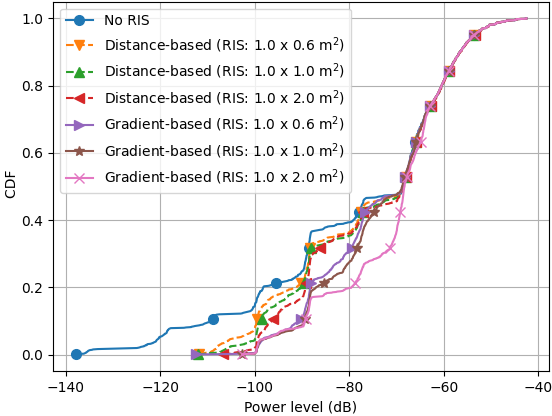
\includegraphics[width=.9\linewidth]{Sim_Results/CDF_-110dB.png}
	\caption{Cumulative distribution functions (CDFs) of power levels for different phase profile approaches and RIS sizes, with a minimum power threshold of $-110$ dB}
	\label{CDF_-110dB}
\end{figure}

The combined coverage maps for the gradient-based and distance-based approaches with a minimum power threshold of $-110$ dB are shown in Figs. \ref{comb_cov_gradient_-110dB} and \ref{comb_cov_distance_-110dB}, respectively. The similar conclusions can be made for the gradient-based approach, it continues to enhance power levels over a broader region. A significant difference is observed for the distance-based approach in Fig. \ref{comb_cov_distance_-110dB}, where full coverage is achieved by focusing on two target points. Compared to the previous case with a $-100$ dB threshold, this setting results in fewer low-power cells concentrated in a smaller blind spot. Consequently, the distance-based approach is particularly effective in scenarios where blind spots are small and all low-power cells are close to the selected target points of the RIS. Ultimately, the updated binary poor coverage maps confirm that full coverage is achieved across the scene.

\begin{figure}
	\centering
	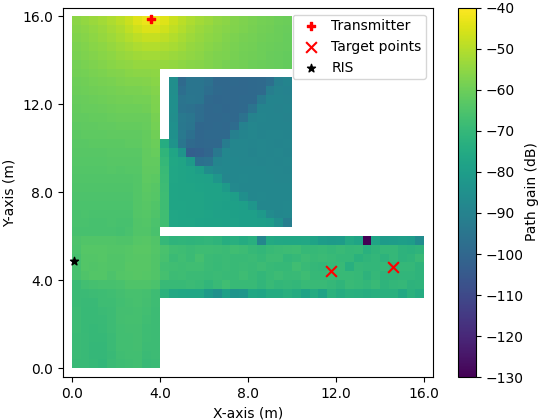
\includegraphics[width=0.8\linewidth]{Sim_Results/Comb_cov_1x2_Gradient_-110dB.png}
	
	a) Combined coverage map \\[5pt]
	
	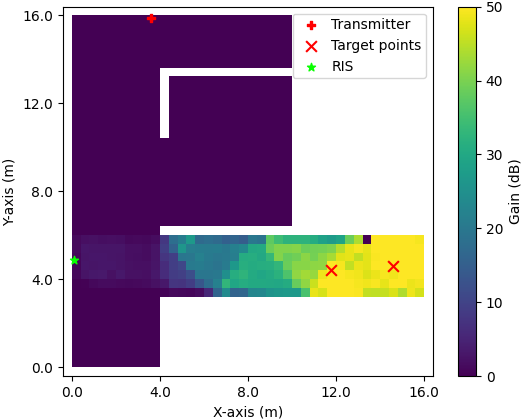
\includegraphics[width=0.49\linewidth]{Sim_Results/RIS_cov_gain_1x2_Gradient_-110dB.png}
	\hfill
	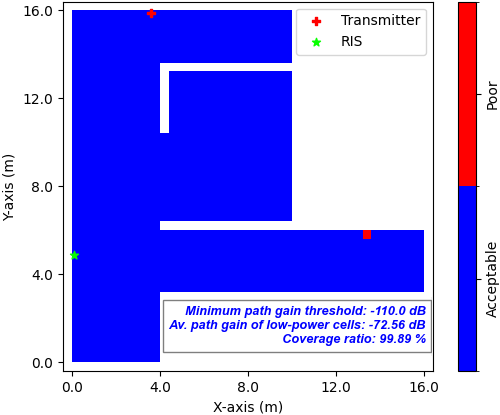
\includegraphics[width=0.48\linewidth]{Sim_Results/New_Binary_Cov_Map_1x2_Gradient_-110dB.png}
	
	\hspace{10pt} b) RIS coverage gain \hspace{30pt} c) Updated binary poor \\ \hspace{140pt} coverage map
	\caption{Combined coverage analysis for a RIS of size $1 \times 2$ m$^2$ using the gradient-based approach, with a minimum power threshold of $-110$ dB}
	\label{comb_cov_gradient_-110dB}
\end{figure}

\begin{figure}
	\centering
	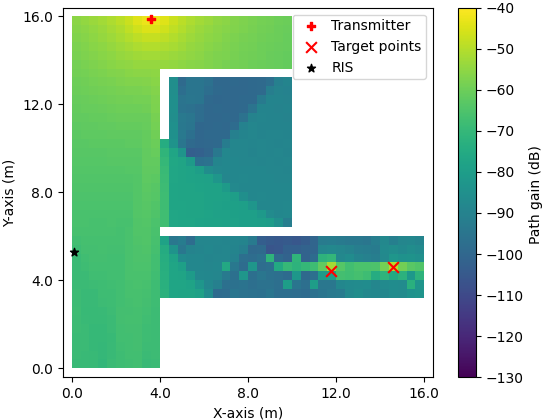
\includegraphics[width=0.8\linewidth]{Sim_Results/Comb_cov_1x2_Distance_-110dB.png}
	
	a) Combined coverage map \\[5pt]
	
	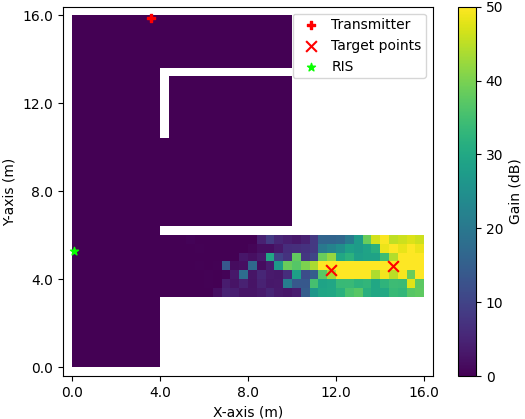
\includegraphics[width=0.49\linewidth]{Sim_Results/RIS_cov_gain_1x2_Distance_-110dB.png}
	\hfill
	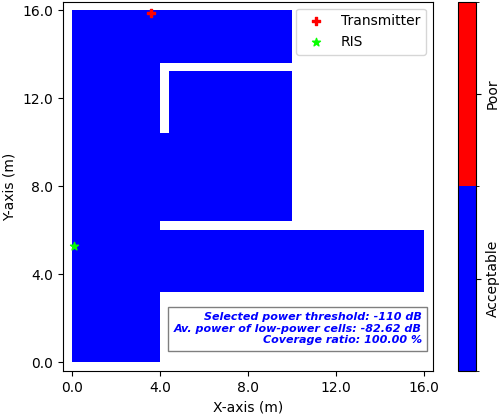
\includegraphics[width=0.48\linewidth]{Sim_Results/New_Binary_Cov_Map_1x2_Distance_-110dB.png}
	
	\hspace{10pt} b) RIS coverage gain \hspace{30pt} c) Updated binary poor \\ \hspace{140pt} coverage map
	\caption{Combined coverage analysis for a RIS of size $1 \times 2$ m$^2$ using the distance-based approach, with a minimum power threshold of $-110$ dB}
	\label{comb_cov_distance_-110dB}
\end{figure}

\section{CONCLUSION} \label{sec:conclusion}
This paper presents a novel ray-tracing-based joint optimization framework for RIS deployment in indoor wireless environments, simultaneously optimizing the RIS position, size, and beam-steering target points. Unlike prior studies that assume fixed RIS positions or arbitrary sizes, our approach systematically determines all key RIS parameters in a unified framework while considering both LoS and non-LoS paths. By integrating ray-tracing simulations with a clustering-based method for identifying target points and a performance-cost trade-off strategy for selecting a sub-optimal RIS size, the proposed method effectively improves coverage and signal quality, especially in blind spots. The simulation results demonstrate that a physically consistent, data-driven optimization approach can significantly enhance indoor communication performance. The findings highlight the importance of optimizing multiple RIS parameters jointly rather than considering them separately, providing a practical methodology for real-world RIS-aided wireless networks. Based on these results, we also propose a general guideline specific to the considered U-shaped indoor office scenario for RIS deployment: (1) the RIS should be mounted on walls with line-of-sight visibility to both the transmitter and all target points, with the optimal location chosen to maximize the performance metric; (2) the RIS size should be increased until the performance improvement drops below a selected performance improvement threshold, enabling size-efficiency trade-offs; and (3) the phase profile configuration method should be selected according to the geometry of the blind-spot region: use the gradient-based approach for broad, dispersed coverage areas where energy needs to be distributed more evenly, and use the distance-based approach for small, confined regions where focused signal enhancement is required. Future work may extend this framework to multi-RIS deployments, where multiple RISs collaboratively optimize coverage over larger indoor areas, further enhancing communication performance in complex propagation environments.

\begin{thebibliography}{00}
	\bibitem{wu_towards} Q. Wu and R. Zhang, “Towards smart and reconfigurable environment: Intelligent reflecting surface aided wireless network," \textit{IEEE Commun. Mag.}, vol. 58, no. 1, pp. 106-112, Jan. 2020.
	\bibitem{e_basar} E. Basar, M. Di Renzo, J. De Rosny, M. Debbah, M. -S. Alouini, and R. Zhang, “Wireless communications through reconfigurable intelligent surfaces," \textit{IEEE Access}, vol. 7, pp. 116753-116773, 2019.
	\bibitem{di_renzo_SRE} M. Di Renzo \textit{et al.}, “Smart radio environments empowered by reconfigurable intelligent surfaces: How it works, state of research, and the road ahead," \textit{IEEE J. Sel. Areas Commun.}, vol. 38, no. 11, pp. 2450-2525, Nov. 2020.	
	\bibitem{elmossalmy} M. A. ElMossallamy, H. Zhang, L. Song, K. G. Seddik, Z. Han, and G. Y. Li, “Reconfigurable intelligent surfaces for wireless communications: Principles, challenges, and opportunities," \textit{IEEE Trans. Cogn. Commun. Netw.}, vol. 6, no. 3, pp. 990-1002, Sept. 2020.
	\bibitem{Wu_IRS_Integre} Q. Wu, S. Zhang, B. Zheng, C. You, and R. Zhang, “Intelligent reflecting surface-aided wireless communications: A tutorial," \textit{IEEE Trans. Commun.}, vol. 69, no. 5, pp. 3313-3351, May 2021.
	\bibitem{path-loss1} Ö. Özdogan, E. Björnson, and E. G. Larsson, “Intelligent reflecting surfaces: Physics, propagation, and pathloss modeling," \textit{IEEE Wireless Commun. Lett.}, vol. 9, no. 5, pp. 581-585, May 2020.
	\bibitem{path-loss2} S. W. Ellingson, “Path loss in reconfigurable intelligent surface-enabled channels," \textit{IEEE 32nd Int. Symp. Pers., Indoor Mobile Radio Commun. (PIMRC)}, Helsinki, Finland, 2021, pp. 829-835.
	\bibitem{Tang} W. Tang \textit{et al.}, “Wireless communications with reconfigurable intelligent surface: Path loss modeling and experimental measurement," \textit{IEEE Trans. Wireless Commun.}, vol. 20, no. 1, pp. 421-439, Jan. 2021.
	\bibitem{pan2021reconfigurable} C. Pan \textit{et al.}, “Reconfigurable intelligent surfaces for 6G systems: Principles, applications, and research directions," \textit{IEEE Commun. Mag.}, vol. 59, no. 6, pp. 14-20, June 2021.
	\bibitem{phase_grad_paper} E. M. Vitucci, M. Albani, S. Kodra, M. Barbiroli, and V. Degli-Esposti, “An efficient ray-based modeling approach for scattering from reconfigurable intelligent surfaces," \textit{IEEE Trans. Antennas Propag.}, vol. 72, no. 3, pp. 2673-2685, Mar. 2024.	
	\bibitem{RISDeploymentComparison} C. You, B. Zheng, W. Mei, and R. Zhang, “How to deploy intelligent reflecting surfaces in wireless networks: BS-side, user-side, or both sides?," \textit{J. Commun. Inf. Netw.}, vol. 7, no. 1, pp. 1-10, Mar. 2022.
	\bibitem{act_passive} C. You and R. Zhang, “Wireless communication aided by intelligent reflecting surface: Active or passive?," \textit{IEEE Wireless Commun. Lett.}, vol. 10, no. 12, pp. 2659-2663, Dec. 2021.
	\bibitem{Wu2019} Q. Wu and R. Zhang, “Intelligent reflecting surface enhanced wireless network via joint active and passive beamforming," \textit{IEEE Trans. Wireless Commun.}, vol. 18, no. 11, pp. 5394-5409, Nov. 2019.
	\bibitem{Wu2019-2} Q. Wu and R. Zhang, “Beamforming optimization for intelligent reflecting surface with discrete phase shifts," \textit{IEEE Int. Conf. Acoust., Speech Signal Process. (ICASSP)}, Brighton, UK, 2019, pp. 7830-7833.
	\bibitem{Wang2020} H. Wang, C. Liu, Z. Shi, Y. Fu, and R. Song, “On power minimization for IRS-aided downlink NOMA systems," \textit{IEEE Wireless Commun. Lett.}, vol. 9, no. 11, pp. 1808-1811, Nov. 2020.
	\bibitem{Abeywickrama2020} S. Abeywickrama, R. Zhang, and C. Yuen, “Intelligent reflecting surface: Practical phase shift model and beamforming optimization," \textit{IEEE Int. Conf. Commun. (ICC)}, Dublin, Ireland, 2020, pp. 1-6.
	\bibitem{DRL1} H. Yang \textit{et al.}, “Intelligent reflecting surface assisted anti-jamming communications: A fast reinforcement learning approach," \textit{IEEE Trans. Wireless Commun.}, vol. 20, no. 3, pp. 1963-1974, Mar. 2021.
	\bibitem{DRL2} K. Feng, Q. Wang, X. Li, and C. -K. Wen, “Deep reinforcement learning based intelligent reflecting surface optimization for MISO communication systems," \textit{IEEE Wireless Commun. Lett.}, vol. 9, no. 5, pp. 745-749, May 2020.
	\bibitem{SecureRIS} M. Cui, G. Zhang, and R. Zhang, “Secure wireless communication via intelligent reflecting surface," \textit{IEEE Wireless Commun. Lett.}, vol. 8, no. 5, pp. 1410-1414, Oct. 2019.
	\bibitem{OptimalRISSize} A. Zappone, M. Di Renzo, X. Xi, and M. Debbah, “On the optimal number of reflecting elements for reconfigurable intelligent surfaces," \textit{IEEE Wireless Commun. Lett.}, vol. 10, no. 3, pp. 464-468, Mar. 2021.
	\bibitem{MultiUserRISSize} H. Zhang, B. Di, Z. Han, H. V. Poor, and L. Song, “Reconfigurable intelligent surface assisted multi-user communications: How many reflective elements do we need?," \textit{IEEE Wireless Commun. Lett.}, vol. 10, no. 5, pp. 1098-1102, May 2021.
	\bibitem{Nguyen2022-1} M. D. Nguyen, L. B. Le, and A. Girard, “UAV placement and resource allocation for intelligent reflecting surface assisted UAV-based wireless networks," \textit{IEEE Commun. Lett.}, vol. 26, no. 5, pp. 1106-1110, May 2022.
	\bibitem{Gu2023-1} X. Gu, G. Zhang, W. Duan, M. Wen, J. Choi, and P. -H. Ho, “ARIS-empowered wireless communications: Joint beamforming design and deployment optimization," \textit{IEEE Wireless Commun. Lett.}, vol. 12, no. 12, pp. 2003-2007, Dec. 2023.
	\bibitem{Nguyen-Kha2022-1} H. Nguyen-Kha, H. V. Nguyen, M. T. P. Le, and O. -S. Shin, “Joint UAV placement and IRS phase shift optimization in downlink networks," \textit{IEEE Access}, vol. 10, pp. 111221-111231, 2022.
	\bibitem{Shang2023-1} B. Shang, E. S. Bentley, and L. Liu, “UAV swarm-enabled aerial reconfigurable intelligent surface: Modeling, analysis, and optimization," \textit{IEEE Trans. Commun.}, vol. 71, no. 6, pp. 3621-3636, June 2023.
	\bibitem{Ge2021-1} L. Ge, H. Zhang, and J. Wang, “Joint placement and beamforming design in multi-UAV-IRS assisted multiuser communication," \textit{IEEE Global Commun. Conf. (GLOBECOM)}, Madrid, Spain, 2021, pp. 1-6.
	\bibitem{Zhou2021-1} T. Zhou, K. Xu, X. Xia, W. Xie, and J. Xu, “Achievable rate optimization for aerial intelligent reflecting surface-aided cell-free massive MIMO system," \textit{IEEE Access}, vol. 9, pp. 3828-3837, 2021.
	\bibitem{Bai2022-1} J. Bai, H. -M. Wang, and P. Liu, “Robust IRS-aided secrecy transmission with location optimization," \textit{IEEE Trans. Commun.}, vol. 70, no. 9, pp. 6149-6163, Sept. 2022.
	\bibitem{Guo2023-1} H. Guo, Z. Yang, Y. Zou, B. Lyu, Y. Jiang, and L. Hanzo, “Joint reconfigurable intelligent surface location and passive beamforming optimization for maximizing the secrecy-rate," \textit{IEEE Trans. Veh. Technol.}, vol. 72, no. 2, pp. 2098-2110, Feb. 2023.
	\bibitem{Aung2024-1} P. S. Aung, Y. M. Park, Y. K. Tun, Z. Han, and C. S. Hong, “Energy-efficient communication networks via multiple aerial reconfigurable intelligent surfaces: DRL and optimization approach," \textit{IEEE Trans. Veh. Technol.}, vol. 73, no. 3, pp. 4277-4292, Mar. 2024.
	\bibitem{Qin2022-1} H. Qin, Z. Liu, and C. Yang, “Indoor mm-wave coverage enhancement: Reconfigurable intelligent surface deployment strategy based on human mobility model," \textit{IEEE Commun. Lett.}, vol. 26, no. 10, pp. 2475-2479, Oct. 2022.
	\bibitem{Feng2025-1} J. Feng, B. Zheng, C. You, P. Chen, X. Xiong, and F. Chen, “6D deployment optimization for intelligent reflecting surface-aided wireless communication," \textit{IEEE Wireless Commun. Lett.}, 2025, doi: 10.1109/LWC.2024.3524592.
	\bibitem{Feng2023-1} J. Feng \textit{et al.}, “Joint passive beamforming and deployment design for dual distributed-IRS aided communication," \textit{IEEE Trans. Veh. Technol.}, vol. 72, no. 10, pp. 13758-13763, Oct. 2023.
	\bibitem{Lu2021-1} H. Lu, Y. Zeng, S. Jin, and R. Zhang, “Aerial intelligent reflecting surface: Joint placement and passive beamforming design with 3D beam flattening," \textit{IEEE Trans. Wireless Commun.}, vol. 20, no. 7, pp. 4128-4143, July 2021.
	\bibitem{Bai2024-1} J. Bai, Q. Yan, H. -M. Wang, and Y. Liu, “Intelligent reflecting surface aided green communication with deployment optimization," \textit{IEEE Trans. Commun.}, vol. 72, no. 8, pp. 5130-5144, Aug. 2024.
	\bibitem{Naeem2023-1} F. Naeem, M. Qaraqe, and H. Celebi, “Joint deployment design and phase shift of IRS-assisted 6G networks: An experience-driven approach," \textit{IEEE Internet Things J.}, vol. 10, no. 20, pp. 17647-17655, Oct. 2023.
	\bibitem{Saqib2023-1} N. U. Saqib, S. Hou, S. H. Chae, and S. -W. Jeon, “RIS-aided wireless indoor communication: Sum rate maximization via RIS placement optimization," \textit{IEEE Int. Conf. Commun. (ICC)}, Rome, Italy, 2023, pp. 511-516.
	\bibitem{Saqib2023-2} N. U. Saqib, S. Hou, S. H. Chae, and S. -W. Jeon, “Reconfigurable intelligent surface aided hybrid beamforming: Optimal placement and beamforming design," \textit{IEEE Trans. Wireless Commun.}, vol. 23, no. 9, pp. 12003-12019, Sept. 2024.
	\bibitem{RISOrientationOptimization} S. Zeng, H. Zhang, B. Di, Z. Han, and L. Song, “Reconfigurable intelligent surface (RIS) assisted wireless coverage extension: RIS orientation and location optimization," \textit{IEEE Commun. Lett.}, vol. 25, no. 1, pp. 269-273, Jan. 2021.
	\bibitem{Rani2024-1} J. Rani, D. Mishra, G. Prasad, A. Hossain, S. De, and K. Deka, “Joint optimization of IRS location and passive beamforming for enhanced received power," \textit{IEEE Trans. Green Commun. Netw.}, vol. 8, no. 4, pp. 1970-1984, Dec. 2024.
	\bibitem{Cheng2022-1} X. Cheng \textit{et al.}, “Joint optimization for RIS-assisted wireless communications: From physical and electromagnetic perspectives," \textit{IEEE Trans. Commun.}, vol. 70, no. 1, pp. 606-620, Jan. 2022.
	\bibitem{Liu2024-1} C. Liu \textit{et al.}, “Reconfigurable intelligent surface assisted high-speed train communications: Coverage performance analysis and placement optimization," \textit{IEEE Trans. Veh. Technol.}, vol. 73, no. 3, pp. 3750-3766, Mar. 2024.
	\bibitem{Zhang2022-1} J. Zhang and D. M. Blough, “Optimizing coverage with intelligent surfaces for indoor mmWave networks," \textit{IEEE Conf. Comput. Commun. (INFOCOM)}, London, United Kingdom, 2022, pp. 830-839.
	\bibitem{Hou2022-1} S. Hou, N. U. Saqib, S. H. Chae, Z. Dou and S. -W. Jeon, “Optimal placement of reconfigurable intelligent surface for millimeter-wave indoor communication," \textit{13th Int. Conf. Inf. Commun. Technol. Convergence (ICTC)}, Jeju Island, Korea, Republic of, 2022, pp. 698-700.
	\bibitem{Mei2023-1} W. Mei and R. Zhang, “Multi-IRS deployment optimization for enhanced wireless coverage: A performance-cost trade-off," \textit{IEEE Int. Conf. Commun. (ICC)}, Rome, Italy, 2023, pp. 2056-2061.
	\bibitem{Mei2023-2} W. Mei and R. Zhang, “Joint base station and IRS deployment for enhancing network coverage: A graph-based modeling and optimization approach," \textit{IEEE Trans. Wireless Commun.}, vol. 22, no. 11, pp. 8200-8213, Nov. 2023.
	\bibitem{Efrem2023-1} C. N. Efrem and I. Krikidis, “Joint IRS location and size optimization in multi-IRS aided two-way full-duplex communication systems," \textit{IEEE Trans. Wireless Commun.}, vol. 22, no. 10, pp. 6518-6533, Oct. 2023.
	\bibitem{Li2022-1} D. Li, “How many reflecting elements are needed for energy- and spectral-efficient intelligent reflecting surface-assisted communication," \textit{IEEE Trans. Commun.}, vol. 70, no. 2, pp. 1320-1331, Feb. 2022.
	\bibitem{Deb2021-1} S. Deb and S. C. Ghosh, “An RIS deployment strategy to overcome static obstacles in millimeter wave D2D communication," \textit{IEEE 20th Int. Symp. Netw. Comput. Appl. (NCA)}, Boston, MA, USA, 2021, pp. 1-8.
	\bibitem{de1} P. -Q. Huang, Y. Zhou, K. Wang, and B. -C. Wang, “Placement optimization for multi-IRS-aided wireless communications: An adaptive differential evolution algorithm," \textit{IEEE Wireless Commun. Lett.}, vol. 11, no. 5, pp. 942-946, May 2022.
	\bibitem{de2} A. Khaled, A. S. Alwakeel, A. M. Shaheen, M. M. Fouda, and M. I. Ismail, “Placement optimization and power management in a multiuser wireless communication system with reconfigurable intelligent surfaces," \textit{IEEE Open J. Commun. Soc.}, vol. 5, pp. 4186-4206, 2024.
	\bibitem{ga1} X. Liu, L. Xue, S. Sun, and M. Tao, “Optimization of RIS placement for satellite-to-ground coverage enhancement," \textit{IEEE Globecom Workshops (GC Wkshps)}, Kuala Lumpur, Malaysia, 2023, pp. 299-304.
	\bibitem{ga2} L. Pang, J. Liu, Y. Zhang, X. Liu, Y. Chen, and A. Wang, “Deployment locations and beamforming optimization for multi-RIS in multi-BS networks," \textit{IEEE 98th Veh. Technol. Conf. (VTC2023-Fall)}, Hong Kong, Hong Kong, 2023, pp. 1-6.
	\bibitem{pso1} M. Misbah, Z. Kaleem, W. Khalid, C. Yuen, and A. Jamalipour, “Phase and 3-D placement optimization for rate enhancement in RIS-assisted UAV networks," \textit{IEEE Wireless Commun. Lett.}, vol. 12, no. 7, pp. 1135-1138, July 2023.
	\bibitem{pso2} H. Lu, H. Zhuang, L. Zhang, and Z. Wang, “Gridding based reconfigurable intelligent surface-aided wireless network optimization," \textit{IEEE 35th Int. Symp. Pers., Indoor Mobile Radio Commun. (PIMRC)}, Valencia, Spain, 2024, pp. 1-6.
	\bibitem{pso3} Q. Chang, G. Nie, H. Tian, G. Li, and B. Zhang, “A sequential-fairness RIS deployment for indoor multi-user systems," \textit{IEEE/CIC Int. Conf. Commun. China (ICCC)}, Dalian, China, 2023, pp. 1-6.
	\bibitem{RT1} Z. Li, O. A. Topal, Ö. T. Demir, E. Björnson, and C. Cavdar, “mmWave coverage extension using reconfigurable intelligent surfaces in indoor dense spaces," \textit{IEEE Int. Conf. Commun. (ICC)}, Rome, Italy, 2023, pp. 5805-5810.
	\bibitem{RT2} A. Albanese, G. Encinas-Lago, V. Sciancalepore, X. Costa-Pérez, D. -T. Phan-Huy, and S. Ros, “RIS-aware indoor network planning: The Rennes railway station case," \textit{IEEE Int. Conf. Commun. (ICC)}, Seoul, Korea, Republic of, 2022, pp. 2028-2034.
	\bibitem{RT3} J. Huang, C. -X. Wang, Y. Sun, J. Huang, and F. -C. Zheng, “A novel ray tracing based 6G RIS wireless channel model and RIS deployment studies in indoor scenarios," \textit{IEEE 33rd Int. Symp. Pers., Indoor Mobile Radio Commun. (PIMRC)}, Kyoto, Japan, 2022, pp. 884-889.
	\bibitem{emre_claude_eucap_paper} E. Kilcioglu and C. Oestges, “Ray-tracing based algorithms for indoor RIS optimization and coverage enhancement," \textit{to appear in 19th European Conf. on Antennas Propag. (EuCAP)}, Stockholm, Sweden, 2025 pp. 1-5.
	\bibitem{sionna} J. Hoydis \textit{et al.}, “Sionna RT: Differentiable Ray Tracing for Radio Propagation Modeling," \textit{IEEE Globecom Workshops (GC Wkshps)}, Kuala Lumpur, Malaysia, 2023, pp. 317-321.
	\bibitem{wireless_insite} Remcom, Inc., Wireless InSite [Computer software], State College, PA, USA. [Online]. Available: https://www.remcom.com/wireless-insite
	\bibitem{ITU} ITU-R, “Recommendation ITU-R P.2040-2: Effects of building materials and structures on radiowave propagation above about 100 MHz," Sep. 2021. [Online]. Available: https://www.itu.int/rec/R-REC-P. 2040-2-202109-I
\end{thebibliography}

\end{document}
